\chapter{Future Work}
\label{sec:futurework}

Tensorflow privacy library \cite{11} provides a function to calculate epsilon based on hyperparameters such as dataset size, batch size, epochs, delta, and noise multiplier. It provides ($\epsilon$,$\delta$)-\text{differential privacy}. But to calculate ($\epsilon$,$\delta$)-\text{differential privacy} with Gaussian and composition rule, the current method is not an accurate fit. To overcome this shorting Rényi divergence is used to measure differential privacy based on paper \cite{23} which provides Rényi Differential Privacy (RDP). It can be applied to calculate privacy loss when composition with heterogeneous mechanisms is involved. Hence, RDP enables us to calculate privacy when sampling distribution along with Gaussian noise is used like in this case. To calculate epsilon it depends upon some hyperparameters as explained below. If any of the below parameters are changed then epsilon value will also change and hence epsilon value can be controlled with the help of these parameters.
\begin{itemize}
    \item \textbf{Dataset Size}: This is the size of the database or dataset.
    \vspace{-0.3cm}\item \textbf{Batch size}: Number of a random sample from the dataset which will be picked up during training in one epoch.
    \vspace{-0.3cm}\item \textbf{Epoch}: Number of training iterations to train the dataset.
    \vspace{-0.3cm}\item \textbf{Delta}: This is the probability of the failure.
\end{itemize}
\end{itemize}


In this thesis, TensorFlow google's opensource framework \cite{24} is used to train models for machine learning. It is known for its flexibility and wide range of libraries and community support to develop machine learning applications. As explained in the last section Google TensorFlow privacy library \cite{11} is used in case the DP flag is chosen as 'noise'. This repository is a library-based in Python and can be used to train various machine learning models with differentially private Tensorflow optimizers such as differentially private Stochastic gradient descent, Adam, Adagrad, etc. If noise is used then optimizers from these libraries are used which will make the model differentially private otherwise optimizers (native non deferentially private) from the Tensorflow framework are used. Based on chosen options above (random response or noise) the model is compiled with the respective loss, optimizer, and input data to yield a model for predictions.

The system consists of a dataset that will be made differentially private (DP) by a randomized response(RR) mechanism or adding a noise and then, trained using the Tensorflow machine learning framework and further integrated with Intel SGX for making it more secure from an adversary. The chosen dataset must be preprocessed to prepare it for the RR mechanism. The training over the dataset explicitly requires tuning hyperparameters. All of this will run inside an enclave which will shield all the data as well as model. 
\section{Design goal}
All or most of the machine learning models are trained using private and sensitive user data. When such models are used in untrusted environments such as public cloud then privacy, as well as security is always the concern. Security here means the confidentiality and integrity of data. To make such a system secure and protect the confidentiality and integrity of a system, Trusted Execution Environment (TEEs) are used for example Intel Software Guard Extension (SGX). This protects the application code and data inside an enclave. But it doesn't provide privacy for data inside an enclave. An advisory can fire many malicious queries for this data hence can breach the privacy of an individual. Hence some privacy mechanism should be used to protect individual's data. This system is designed keeping in mind the following goals :
\begin{itemize}
  \item \textbf{Security}: The security concern is addressed using Intel SGX.
  \vspace{-0.3cm}\item \textbf{Privacy}: Privacy concern for protecting individual's data is addressed using differential privacy.
  \vspace{-0.3cm}\item \textbf{Transparency}: System should be easy to access and use with minimum or no code changes hence APIs should be exposed for the usage of the system.
  \vspace{-0.3cm}\item \textbf{Scalability}: It must be easy to scale up the resources of the system. This will be achieved using docker and additionally the machine learning framework should support distributed learning.
  \vspace{-0.3cm}\item \textbf{Performance}: Performance should be the same as the native performance with as little overhead as possible.
  \vspace{-0.3cm}\item \textbf{Accuracy}: Accuracy should be the same as native accuracy with as little overhead as possible.
\end{itemize} 
\section{System Architecture}
The system mainly consists of a user, dataset, machine learning framework and an Intel SGX memory or enclave as the main components as shown in Figure 4.1.
\begin{itemize}
    \item \textbf{Users}
The users of this system are human users or some scripts to make predictions. Users can be a direct consumer or some administrator or technician supporting the maintenance of the system. Each user is authorized to use the system and is enrolled as part of some organization. 
    \vspace{-0.3cm}\item \textbf{TEEs-Intel SGX}
Intel SGX is used for a trusted execution environment here. Enclaves are created as private memory regions that contain sensitive data and code. No process outside it can read or save anything in enclaves. This will provide confidentiality and integrity to the system.
    \vspace{-0.3cm}\item \textbf{Dataset}
The dataset here stands for training data on which training computation needs to be performed. Dataset may be maintained as a directory structure, CSV file or HDF5 file, etc. If the dataset needs to be kept outside the enclave it will be in encrypted form. This is the data where security and privacy is required to protect it against any kind of data leak.
    \vspace{-0.3cm}\item \textbf{Differential Private Module}
This module contains a mechanism to make the dataset differentially private to provide privacy on an individual's data. There are many perturbations techniques available to achieve differential privacy such as input, output, objective, and gradient perturbations. In this thesis, the input perturbations mechanism based on a randomized response is used. The objective perturbations based on the Google Tensorflow Privacy library is also explored as part of this thesis. It adds Gaussian noise at each gradient function. A flag is used to control which type of DP module should be selected. 
    \vspace{-0.3cm}\item \textbf{Machine learning framework}
There are a lot of machine learning frameworks available to develop and train models such as Pytorch, Tensorflow, Scikit-learn library, etc. In this thesis, TensorFlow google's opensource framework is used to train models for machine learning. It is known for its flexibility and wide range of libraries and community support to develop machine learning applications.
    \vspace{-0.3cm}\item \textbf{Machine learning model}
A machine learning model aims to find a correlation between input parameters also known as features and output parameters known as labels in the training set. Different types of models can be used such as CNN (Convolutional Neural Networks), RNN(Recurrent Neural Networks), or Linear Regression depending upon the type of the dataset in question. Depending upon the chosen framework, machine learning model will be defined with respective loss and optimizer functions. 
    \vspace{-0.3cm}\item \textbf{Privacy preserving model}
The privacy-preserving model is a trained model on the respective differential private dataset. This model provides security using TEEs and privacy using differential privacy hence preventing any kind of data leakage.
    \vspace{-0.3cm}\item \textbf{Prediction}
It takes input from the user which is not known to the model and pass it on to the trained model to predict the target output. The model publish its prediction based on the training it has done on the trained data and tried the predict the best possible outcome from the test data.
\end{itemize}
\begin{figure}
    \centering
    \includegraphics[width=10cm, height=10cm]{images/Slide1.png}
    \caption{System Design}
    \label{default}
\end{figure}

\section{Threat Model}
In this threat model, the dataset, model, and an application are inside the SGX memory hence making it secure in terms of confidentiality and integrity. Privacy of the data especially against malicious queries is protected by differential privacy. Users can be trusted most of the times but sometimes an adversary might attack the system through inversion attacks i.e black-box queries which might training data. Two types of black-box attacks can be used to learn individual's data, membership inversion attack, and model inversion attack as explained in background section 3.8.1 and 3.8.1. So even with the help of these attacks an adversary will be learning information from a differentially private dataset which will contain random information instead of actual information, hence protecting the privacy of an individual.

If an attacker can get access to the system components or get root privileges then also code, data, and application are running inside an enclave, which would be nearly impossible to break the security primitives. The SGX enclaves also protect code and application inside enclaves against any non trusted OS. The only attack possible is to physically tamper the system, which is also not possible to trace out the exact location of the system and more importantly enter the premises.

Additionally, TEEs are prone to side-channel attacks, these things are not explored as part of this thesis.
\section{System Detail}
The system consists of two phases(1) Training phase (2) Inference phase
\subsection{Training phase}
For this phase, the dataset acts as an input, and output is a differentially private model. The data is scattered sometimes in different files or just one CSV file or HDF5 compressed file. As depicted from the APIs flow in Figure 4.2, \textit{getData()} is used to populate data into respective variables depending upon the type of the dataset used. After loading data the next step is to preprocess the dataset. The \textit{dpFlag()} enables the selection of the type of differential private setting that is random response or noise. For the random response to work, the data should be numeric so preprocessing on data columns is required to convert an object or categorical data columns into numeric ones. API \textit{preprocessData()} does this job. The dataset(full or some sensitive columns) is randomized using differentially private module  \textit{rr(column,p,q)}. p and q are the probability bias which are covered later in the detail. This module uses local DP based on a randomized response technique \cite{14}. For noise, the dataset itself is not made differentially made private but instead noise is added during the training process in the objective or gradient functions. Google TensorFlow privacy library \cite{11} can be used to fulfill this type of differential privacy requirement and is based on global DP. This repository is a library-based in Python and can be used to train various machine learning models with differentially private Tensorflow optimizers such as differentially private Stochastic gradient descent, Adam, Adagrad, etc. If noise is used then optimizers from these libraries are used which will make the model differentially private. Based on chosen options above \textit{defineModel()} compiles all the required parameters such as loss function, training dataset, \textit{optimizer()} or \textit{dpOptimizer()} depending upon \textit{dpFlag()}. There are many options available for loss function and it is highly dependent upon the type of the problem being solved here. For optimizers, most of the time Gradient descent optimizer is used but there are many other options available. The model is compiled and trained to generate a differentially private model which can then be used for doing predictions. 

\begin{figure}
    \centering
    \includegraphics[width=10cm, height=10cm]{images/Slide2.png}
    \caption{APIs Flow}
    \label{default}
\end{figure}
\subsection{Inference phase}
In phase2, the differentially private model is used for making predictions. The training phase gives us a trained model \textit{ppTrainedModel()}
to do the predictions. These predictions can be a binary or image classifications. Users as shown in Figure 4.2 submit the test data on the model to make predictions using \textit{predict()}. The input from \textit{predict()} is passed to \textit{ppTrainedModel()} which will evaluate test data against trained model and will predict the target output.

\begin{table}[h!]
  \begin{center}
    \caption{MNIST Latency Comparison}
    \label{tab:table}
    \begin{tabular}{l|l|l|l}
      \textbf{Epsilon} & \textbf{Noise1(sec)} & \textbf{Noise2(sec)} & \textbf{Noise1+Noise2(sec)}\\
      \hline
0.1 &		7.133851004 &		1031.587144 &		928.7132077\\
1 &		7.436668205 &		1057.636842 &		955.9761744\\
2 &		7.929595971 &		927.3446046 &		987.846331\\
4 &		8.512832499 &		995.9816808 &		1066.971232\\
6 &		9.029140472 &		888.2222818 &		987.3786404\\
8 &		9.519301558 &		885.6387458 &		883.374013\\
Baseline &		6.318432188 &		6.318432188 &		6.318432188\\
    \end{tabular}
   \end{center}
\end{table}



\begin{table}[h!]
  \begin{center}
    \caption{Cifar10 Latency Comparison}
    \label{tab:table}
    \begin{tabular}{l|l|l|l}
      \textbf{Epsilon} & \textbf{Noise1(sec)} & \textbf{Noise2(sec)} & \textbf{Noise1+Noise2(sec)}\\
      \hline
0.1&	9.26152496&	1289.147366&	992.6722354\\
1&	10.57319551&	1218.083061&	1039.126912\\
2&	11.88289256&	1148.348852&	1004.607525\\
4&	13.20964863&	1056.939882&	1032.650194\\
6&	14.46581542&	1363.514831&	1059.24401\\
8&	15.97985888&	1006.634384&	1032.863536\\
Baseline&	8.918969321	&8.918969321&	8.918969321\\      
    \end{tabular}
   \end{center}
\end{table}
\cleardoublepage


\cleardoublepage


 The intermediate output after the training of the model will be \textbf{Encrypted privacy preserving model}. The privacy-preserving model is a trained model on the respective input data after the training phase. This will be used along with the input test data to produce the final output encrypted inference result, these are the actual predictions one is interested in. These also contain sensitive information so when SPML coughs out the final output inside an enclave it will be in plain text and when this result is saved on a filesystem it will be saved in an encrypted form to prevent any security breach or leakage.
\begin{figure}
    \centering
    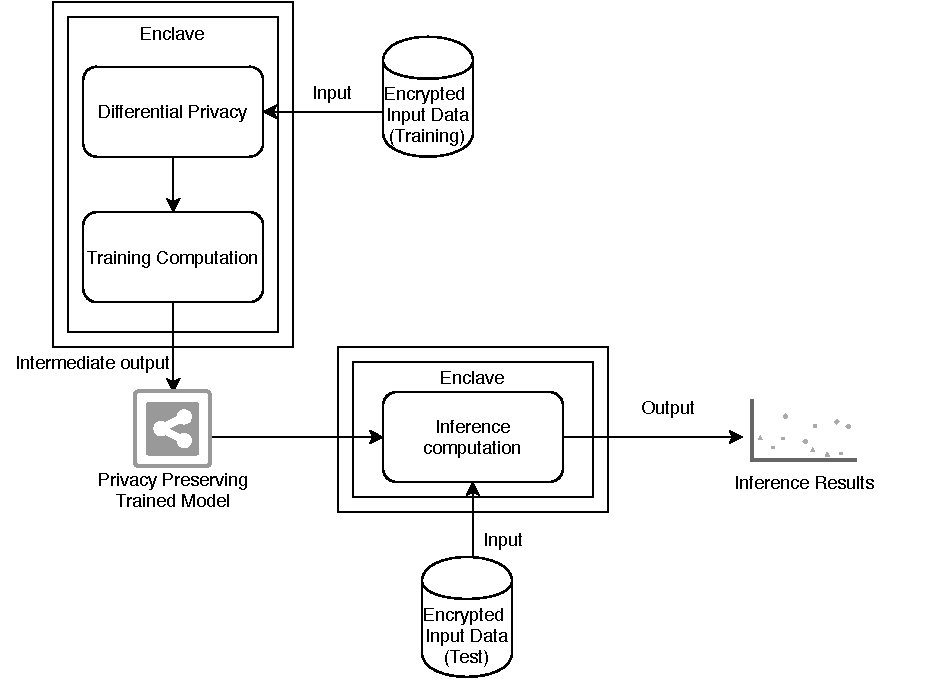
\includegraphics[width=10cm, height=10cm]{images/HLD.jpg}
    \caption{ High-level design}
    \label{default}
\end{figure}
SPML consists of three major components discussed below. The majority of the computation takes place inside an enclave (TEE) which aims to provide security to application code and data. The privacy computation is also done inside an enclave on the input data. TEEs here not only provide just the execution environment but it plays a major role in protecting the data and preserve its confidentiality and integrity end to end.
\begin{itemize}
    \item \textbf{Differential privacy}
This module contains a mechanism to make the input training data differentially private to provide privacy on an individual's data. There are many perturbations techniques available to achieve differential privacy such as input, output, objective, and gradient perturbations. Each of the perturbation techniques follows its advantages and disadvantages. These perturbations techniques work by adding noise over the input data. These are special noises such as Laplace noise, Gaussian noise or randomized response, etc. These noises are added in a way such that computations can be correctly performed and privacy of the data is also preserved. The module is executed inside TEEs to provide security to the application code and data.
    \vspace{-0.3cm}\item \textbf{Training computation}
This module is the main computation module for training the input data. The training can be either using machine learning or deep learning mechanisms. It is kind of a wrapper that can be called using APIs without changing much of the existing machine learning functionality hence provide transparency and easy use of features of the SPML system. All the training computation takes in TEEs hence it is always secured. 
    \vspace{-0.3cm}\item \textbf{Inference computation}
It takes input data (test data) which is not known to the model and privacy-preserving trained model (intermediate output of the training phase) to predict the target output. These computations take place in TEEs to protect the data. The input test data is also kept in an encrypted form on the filesystem to protect its confidentiality and integrity. The model publishes its prediction based on the training it has done on the trained data and tries to predict the best possible outcome from the test data and the output from this computation is also encrypted making it secure and private.
\end{itemize}


\chapter{Evaluation}
\label{sec:eval}
In this section, SPML will be evaluated in terms of efficiency, accuracy, latency and security. The details about the experimental setup used, the data set used, and the methodology followed will be discussed. To conduct experiments TensorFlow privacy library \cite{11} is used. This library adds noise from Gaussian distribution during training of dataset. The effect of differential privacy on native machine and running it with hardware in SCONE runtime ennvironment will be evaluated.

\section{Experimental Setup}
To evaluate \dip, google's open-source TensorFlow privacy library is used. The repository \cite{11} is a library based in Python and can be used to train various machine learning models with differentially private Tensorflow optimizers such as differentially private Stochastic gradient descent, Adam, Adagrad, etc. Additionally, it also provides tools to compute the privacy achieved using these optimizers. TensorFlow privacy library \cite{11} version 0.2.2 was used as an underlying library for \dip. TensorFlow version 1.15 was used with Keras version 2.3.1. 
\subsection{Testbed}
The machine used for running experiments was linux with 2.2 GHz Quad-Core Intel(R) Xeon(R) CPU E3-1280 v6 @ 3.90GHz with 8 cores and RAM as 64 GB. 
\subsection{Methodology}
SCONE supports two mode simulation mode and actual hardware mode. The tests are conducted for three modes (1) Native mode without SCONE (and without Intel SGX) (2) Sim Mode with SCONE (and without Intel SGX) (3) Hardware mode with SCONE (and with Intel SGX). Tests are conducted for non DP mode and DP mode for MNIST and CIFAR10 dataset. In non DP mode, optimizers from Tensorflow libraries are used and for DP mode, optimizers from Tensorflow privacy libraries are used. For training phase the final accuracy and latency score is an average of 10 iterations with 5 epochs for each epsilon value.
\section{MNIST}
The MNIST is a handwritten digits database\cite{12}. The original set has 60,000 training example but for this experiment, this dataset is reduced to use 10,000 examples for training phase. These images are greyscaled and centered in a 28x28 image. For inference phase, dataset of 10,000 images from the original set is extracted and used to evaluating trained model.
\begin{figure}
     \begin{subfigure}{0.5\textwidth}
         \includegraphics[width=\textwidth]{images/MNIST_accuracy.png}
         \caption{Accuracy}
         \label{default}
     \end{subfigure}
     \begin{subfigure}{0.5\textwidth}
         \includegraphics[width=\textwidth]{images/MNIST_latency.png}
         \caption{Latency}
         \label{default}
     \end{subfigure}
        \caption{Accuracy and latency MNIST Dataset - Native}
        \label{default}
\end{figure}

\begin{figure}
     \begin{subfigure}{0.5\textwidth}
         \includegraphics[width=\textwidth]{images/MNISTHW_accuracy.png}
         \caption{Accuracy}
         \label{default}
     \end{subfigure}
     \begin{subfigure}{0.5\textwidth}
         \includegraphics[width=\textwidth]{images/MNISTHW_latency.png}
         \caption{Latency}
         \label{default}
     \end{subfigure}
        \caption{Accuracy and latency MNIST Dataset - Hardware}
        \label{default}
\end{figure}

The first metric is to see how accuracy is varied with epsilon. For all three variations noise1, noise2 and their combination accuracy increases as the epsilon value is increased. For noise1 the lower accuracy achieved was almost 11 percent and the highest was 88 percent. For small values of epsilon noise added is higher hence the accuracy achieved is bad. For noise2 the accuracy was almost the same and varied mostly between 76-77 percent. Upon combining both the noises the accuracy increases as epsilon is increased for both the noises. At some points for noise2 especially at epsilon values 2 and 4, the accuracy showed a slight decrease as compared to epsilon value 1. The reason for this is that here a subset of actual MNIST set is used. Figure 4.4 shows the details for accuracy at all noises for each epsilon value.

The second metric is epsilon vs latency, baseline, and noise1 shows the almost comparable time while noise2 and combination show almost comparable results. It can be concluded from Table 4.3 that latency has little or no effect with the noise level.

\section{Cifar10}
The Cifar10 database\cite{13} has 50000 32x32 training images. These images belong to 10 classes such as airplanes, automobiles, birds, etc. For this experiment, 3000 images are chosen for training and test data.
\subsubsection{Result}
\begin{figure}
     \begin{subfigure}{0.5\textwidth}
         \includegraphics[width=\textwidth]{images/Cifar10_accuracy.png}
         \caption{Accuracy}
         \label{default}
     \end{subfigure}
     \begin{subfigure}{0.5\textwidth}
         \includegraphics[width=\textwidth]{images/Cifar10_latency.png}
         \caption{Latency}
         \label{default}
     \end{subfigure}
        \caption{Accuracy and latency Cifar10 Dataset - Native}
        \label{default}
\end{figure}

\begin{figure}
     \begin{subfigure}{0.5\textwidth}
         \includegraphics[width=\textwidth]{images/Cifar10hwaccuracy.png}
         \caption{Accuracy}
         \label{default}
     \end{subfigure}
     \begin{subfigure}{0.5\textwidth}
         \includegraphics[width=\textwidth]{images/Cifar10hwlatency.png}
         \caption{Latency}
         \label{default}
     \end{subfigure}
        \caption{Accuracy and latency Cifar10 Dataset - Hardware}
        \label{default}
\end{figure}

The first metric accuracy vs epsilon, for noise1 the lower accuracy achieved was almost 11 percent and the highest was 28 percent. For noise2 also the accuracy varies from 10 percent to 16 percent. Upon combining both the noises the accuracy increases as epsilon increases for both the noises. At some points for noise2 especially at epsilon value 4, the accuracy showed a slight decrease as compared to epsilon value 2. The reason for this is that here a subset of actual Cifar10 set is used. Figure 4.5 shows the details for accuracy at all noises for each epsilon value. The graphs here indicate the same conclusion as graphs for the MNIST dataset which is accuracy increases as epsilon value increases.

The second metric is epsilon vs latency, baseline, and noise1 shows the almost comparable time while noise2 and combination show almost comparable results. It can be concluded from Table 4.4 that latency has little or no effect with the noise level.

We will add privacy , confidentiality and integrity to this machine learning module. Confidentiality and security aspects are addressed using TEEs. There are many other techniques also to provide confidentiality and integrity to the system such as homomorphic encryption. However, homomorphic encryption suffers from the problem of high latency and limited operation. TEEs on other hand are more practical in terms of performance and can support up to many operations hence, we decided to use TEEs for adding confidentiality and integrity to our system. To ensure privacy, differential privacy technique \cite{3} is used so that no information is leaked per individual. 

There are many related works proposed in the area of machine learning to preserve privacy, some of these are discussed below. This section is organized by discussing first related work for machine learning and differential privacy together then the focus will be on state of art privacy-preserving machine learning techniques which is proposed by Google, deep learning with differential privacy which adds Gaussian noise. Google also proposed RAPPOR based on randomized response to achieve differential privacy which will be studied to understand the difference between various techniques that exist for differential privacy.

\section{RAPPOR: Randomized Aggregatable Privacy-Preserving Ordinal Response}
This paper talks about the start of the art method of achieving differential privacy using Randomized Response. RAPPOR \cite{5}, most of the chrome users face an issue wherein an attacker wants to change the default home page on the browser but to find more about this type of attack, one needs to know what kind of homepages are used by the users which means invading the privacy of the user. The approach is to find an algorithm that aims to find popular percentages of homepages or search engines like yahoo, bing, google, etc being used and to see if some attack is found out in this process. RAPPOR finds the distribution of search engines without compromising the security of a particular user. It implements privacy to learn user statistics by imposing privacy guarantees for each user, user data is not maintained in some database, unlike other use cases hence there is no third party involved to put the trust into. 

The first step is to use Bloom Filters to represent URLs.But blooms filters have collisions which means they can report false positives and to solve this problem a concept of the cohort is used. These cohorts are randomly chosen based on some ID of the user say Gmail ID and then the particular set of bloom filters are assigned to this cohort. To summarize this, URLs are converted to bloom filters and a subset is chosen from a big bit vector, and noise is added there. But most of this data is needed in almost real-time, which means data is collected frequently which means an adversary can learn about the user(true value) if the same data is collected again and again. So true value data say B should be replaced by some randomized value B'. This is done with the help of a Permanent randomized response mechanism wherein B' is a binary representation of actual value B based on the randomization technique based on probability. Later this value B' is memoized until actual value changes. With this, the adversary cannot know true and noisy values (i.e B and B'), and averaging attack can be avoided which states that by observing the multiple version of noise value, true value can be deduced.B' can be seen as a unique ID and hence there could be a longitudinal attack over it. In this type of attack, an attacker tracks or generates multiple reports for the same user and if the underlying value which is B' in our case is not changing much, then all the client's reports can be accessed. The second randomization is randomizing the B' from the last step to make it more difficult to guess. Both Permanent and Instantaneous randomized responses satisfied differential privacy as proved in the paper \cite{5}.

The RAPPOR requires a lot of parameters to be specified to achieve privacy for the one-time or longitudinal report and these parameters should be specified cautiously and correct. A user can log in through different devices like phone, PC, tablet, etc which may lead to another problem of information leakage if all these data is collected for a single event. Also, the number of the cohort (subset chosen from big vector) must be changed as it may help to track the clients and can reduce privacy. Hence RAPPOR helps in anonymous data collection, ensures privacy guarantees to data, and omits the third party maintenance of this data.

But if there are fewer samples, this usually results in bad accuracy. To add this randomization to the (chosen) dataset, some columns are chosen and random noise is added to that. For example, if an adult dataset \cite{15}, is taken into consideration with size as 39040 for training and 9792 as validation. It's predicting if total income > 50K/yr based on data like age, work-class, education, education-num, marital status, occupation, sex, etc. Noise can be added in all or some columns, let's assume noise is added to any two columns say work-class, sex or Martial status, and income before training the algorithm with the TensorFlow framework. 

\subsection{Types of Differential Privacy}
Two types of Differential privacy exist local differential privacy and global differential privacy. These both differ with each other based on the place where noise is added. In this thesis, the noise is added on a statistical survey dataset such as an adult dataset \cite{15} before training via local differential privacy and during training via global differential privacy to understand the effect of both of these noise on accuracy and latency of training the model using machine learning.

\subsubsection{Local Differential Privacy}
In this type of differential privacy, noise is added to each data point, which means data is randomized before saving it to the database. Here technique, as proposed by Warner \cite{14}, is used which is based on a coin flip. According to this technique, randomness is added to the response by each person. If simple questions are asked which can be answered in yes/no then according to Warner (1) A coined is flipped two times (2) If its head question is honestly answered (3) If its tail, then second coin flip comes into play :(a) Yes is answered for the head (b) No is answered for the tail. This is also known as plausible deniability. But if there are fewer samples, this usually results in bad accuracy. To add this randomization to the (chosen) dataset, some columns are chosen and random noise is added to that. For example, if an adult dataset \cite{15}, is taken into consideration with size as 39040 for training and 9792 as validation. It's predicting if total income > 50K/yr based on data like age, work-class, education, education-num, marital status, occupation, sex, etc. Noise can be added in all or some columns, let's assume noise is added to any two columns say work-class, sex or Martial status, and income before training the algorithm with the TensorFlow framework. The advantage of using this type of noise is that it is easy to implement but the major disadvantage is that, to add randomization each dataset must be studied and re-engineered/pre-processed to add random noise to it.

\subsubsection{Global Differential Privacy}
Here noise is added once to the output as opposed to local differential privacy where noise is added at each data point. This is known to result in better accuracy. To evaluate differential privacy, google's open-source TensorFlow privacy library \cite{11} is used which adds Gaussian noise at the output of the dataset during training the model. If the same adult dataset is taken into consideration then the noise is added during the training process here. The input data points are not changed at all and data is fed as it is to the model. By varying different noise values, epsilon value will be varied to see the effect on accuracy. The advantage of using this type of differential privacy is that the baseline dataset doesn’t need to be re-engineered and by just changing the optimizer in the machine learning model, differential privacy can be achieved. But to implement this type of privacy, knowledge of computational mathematics is required to add noise at the output.

\section{Randomized response}
To evaluate randomized response technique same experimental setup as discussed in 6.1 is used. The only difference is instead of average of 10 iterations over 5 epochs for each epsilon, 10 iteration is averaged over 50 epochs. The adult dataset \cite{15} is used to implement randomized response with size 39040 for training and 9792 as inference. The measurements are run for all three modes i.e native, simulation and hardware mode for both training and inference phases. Now we will look into these results detail.



Let's assume after randomization, total yes answers are represented by $R_y$, and N is the total answers. To calculate original yes $O_y$ is calculated as :
\begin{equation}
O_y = \frac{R_y - (1 - p) * q * N}{p}
\end{equation}
$O_y$ is calculated using the above formula and let $A_y$ are the actual answers before randomized response then accuracy loss 'L' is calculated as:
\begin{equation}
L = \left|{\frac{A_y-O_y}{A_y}}\right|
\end{equation}
%\cleardoublepage


Executing hardware with TEEs will add little overhead in latency and performance but this is acceptable as one is getting security without changing anything in the current system which is cost-effective and a lot of time will be saved making each application secure. Hence, SPML has very less overhead overall and can be easily deployed in any cloud environment without changing much of the existing code. 



\section{SCONE FSPF}
To provide encryption/decryption a pair of cryptographic keys is needed by an enclave. However, this pair cannot be kept in memory and need to be saved locally on a filesystem. SCONE FSPF is File System Protection File that is responsible for encrypting files stored on a file system. Integration with SCONE FSPF is also needed to make the SPML system ready for deployment.

\section{Implementation of machine learning attacks}
As discussed in the background chapter, we have discussed privacy attacks on machine learning and differential privacy has been proven to be a preventive measure for these types of attacks. As an enhancement and verification step, we can implement these attacks and run these after training models to see if our system SPML can prevent such attacks.

\begin{table}[h!]
  \begin{center}
    \caption{MNIST Accuracy Comparison}
    \label{tab:table}
    \begin{tabular}{l|l|l|l}
      \textbf{Epsilon} & \textbf{Native(sec)} & \textbf{Simulation(sec)} & \textbf{Hardware(sec)}\\
      \hline
0.1 &        12.55999953 &        11.9099997 &        8.259999752\\
1 &        21.18999958 &        30.45000136 &        33.75999928\\
2 &        63.77999783 &        62.41000295 &        63.98000121\\
4 &        74.57000017 &        77.21999884 &        78.04999948\\
6 &        81.43000007 &        80.50000072 &        78.92000079\\
8 &        85.14999747 &        79.43000197 &        84.60999727\\
native TensorFlow &        92.6699996 &        79.35000062 &        88.01000118\\
    \end{tabular}
   \end{center}
\end{table}
\begin{table}[h!]
  \begin{center}
    \caption{MNIST Latency Comparison}
    \label{tab:table}
    \begin{tabular}{l|l|l|l}
      \textbf{Epsilon} & \textbf{Native(sec)} & \textbf{Simulation(sec)} & \textbf{Hardware(sec)}\\
      \hline
0.1 &        0.289653087 &        0.680645418 &        1.948057604\\
1 &        0.287622118 &        0.685371685 &        2.009140778\\
2 &        0.28791244 &        0.690530086 &        1.933781958\\
4 &        0.288543868 &        0.684112549 &        1.99071703\\
6 &        0.288737249 &        0.685911727 &        1.952671814\\
8 &        0.288944864 &        0.686230779 &        1.931935406\\
native TensorFlow &        0.292551422 &        0.685883307 &        1.976682448\\
    \end{tabular}
   \end{center}
\end{table}




\subsection{Inference}
\begin{table}[h!]
  \begin{center}
    \caption{CIFAR10 Accuracy Comparison}
    \label{tab:table}
    \begin{tabular}{l|l|l|l}
      \textbf{Epsilon} & \textbf{Native(sec)} & \textbf{Simulation(sec)} & \textbf{Hardware(sec)}\\
      \hline
0.1 &        9.633333236 &        10.23333296 &        9.966666996\\
1 &        10.36666632 &        10.1333335 &        10.06666645\\
2 &        9.966666996 &        9.533333033 &        9.499999881\\
4 &        10.23333296 &        9.633333236 &        9.966666996\\
6 &        9.566666931 &        9.566666931 &        10.00000015\\
8 &        8.96666646 &        10.00000015 &        9.600000083\\
native TensorFlow &        10.19999981 &        9.933333099 &        10.30000001\\    
    \end{tabular}
   \end{center}
\end{table}
\begin{table}[h!]
  \begin{center}
    \caption{CIFAR10 Latency Comparison}
    \label{tab:table}
    \begin{tabular}{l|l|l|l}
      \textbf{Epsilon} & \textbf{Native(sec)} & \textbf{Simulation(sec)} & \textbf{Hardware(sec)}\\
      \hline
0.1 &        0.304030609 &        0.791026998 &        5.807478404\\
1 &        0.305371594 &        0.7969033 &        5.779322529\\
2 &        0.303365946 &        0.794456339 &        5.921590924\\
4 &        0.305403352 &        0.797351193 &        5.838274264\\
6 &        0.304973602 &        0.799707961 &        5.848085451\\
8 &        0.305365777 &        0.790111113 &        5.845694613\\
native TensorFlow &        0.306777811 &        0.795679665 &        5.801341677\\
    \end{tabular}
   \end{center}
\end{table}


\begin{table}[h!]
  \begin{center}
    \caption{Randomized response accuracy comparison}
    \label{tab:table}
    \begin{tabular}{l|l|l|l}
      \textbf{Epsilon} & \textbf{Native(sec)} & \textbf{Simulation(sec)} & \textbf{Hardware(sec)}\\
      \hline
     
0.13 &        79.75923419 &        81.22832179 &        76.36196613\\
0.53 &        76.33135915 &        81.40175343 &        81.89145327\\
1 &        76.85166001 &        76.37217045 &        77.19852924\\
2 &        81.91185594 &        75.03570914 &        76.37217045\\
3 &        68.74107122 &        71.17934823 &        81.77922964\\
4 &        75.93348026 &        81.24872446 &        81.12630248\\
native TensorFlow &        80.76922894 &        72.15874195 &        82.78922439\\
    \end{tabular}
   \end{center}
\end{table}
\begin{table}[h!]
  \begin{center}
    \caption{Randomized response latency comparison}
    \label{tab:table}
    \begin{tabular}{l|l|l|l}
      \textbf{Epsilon} & \textbf{Native(sec)} & \textbf{Simulation(sec)} & \textbf{Hardware(sec)}\\
      \hline
0.1 &        0.29410789 &        0.549331856 &        1.620006466\\
1 &        0.280151153 &        0.435758233 &        1.620862556\\
2 &        0.296003222 &        0.485510612 &        1.630309582\\
4 &        0.297162724 &        0.486036777 &        1.625596356\\
6 &        0.298868418 &        0.55124011 &        1.6261516811\\
8 &        0.303794694 &        0.549147987 &        1.622182918\\
native TensorFlow &        0.279120398 &        0.543013215 &        1.881222868\\
    \end{tabular}
   \end{center}
\end{table}


%\bibliography{own.bib}
%\fi
%\cleardoublepage
%\addappheadtotoc
%\appendix
%\section{Model inversion attack - images}
\label{sec:MIA}
In section ~\ref{sec:attackOnML}, we have discussed about the model inversion attack on machine learning systems. We showed images only for native Tensorflow trained model, and differentially private model with epsilon values 0.2 and 8 in section 6.5. The complete images we got from trained model with different epsilon values are shown in Figure A.1, A.2 and A.3.
\begin{figure}[h!]
     \begin{subfigure}{.325\textwidth}
         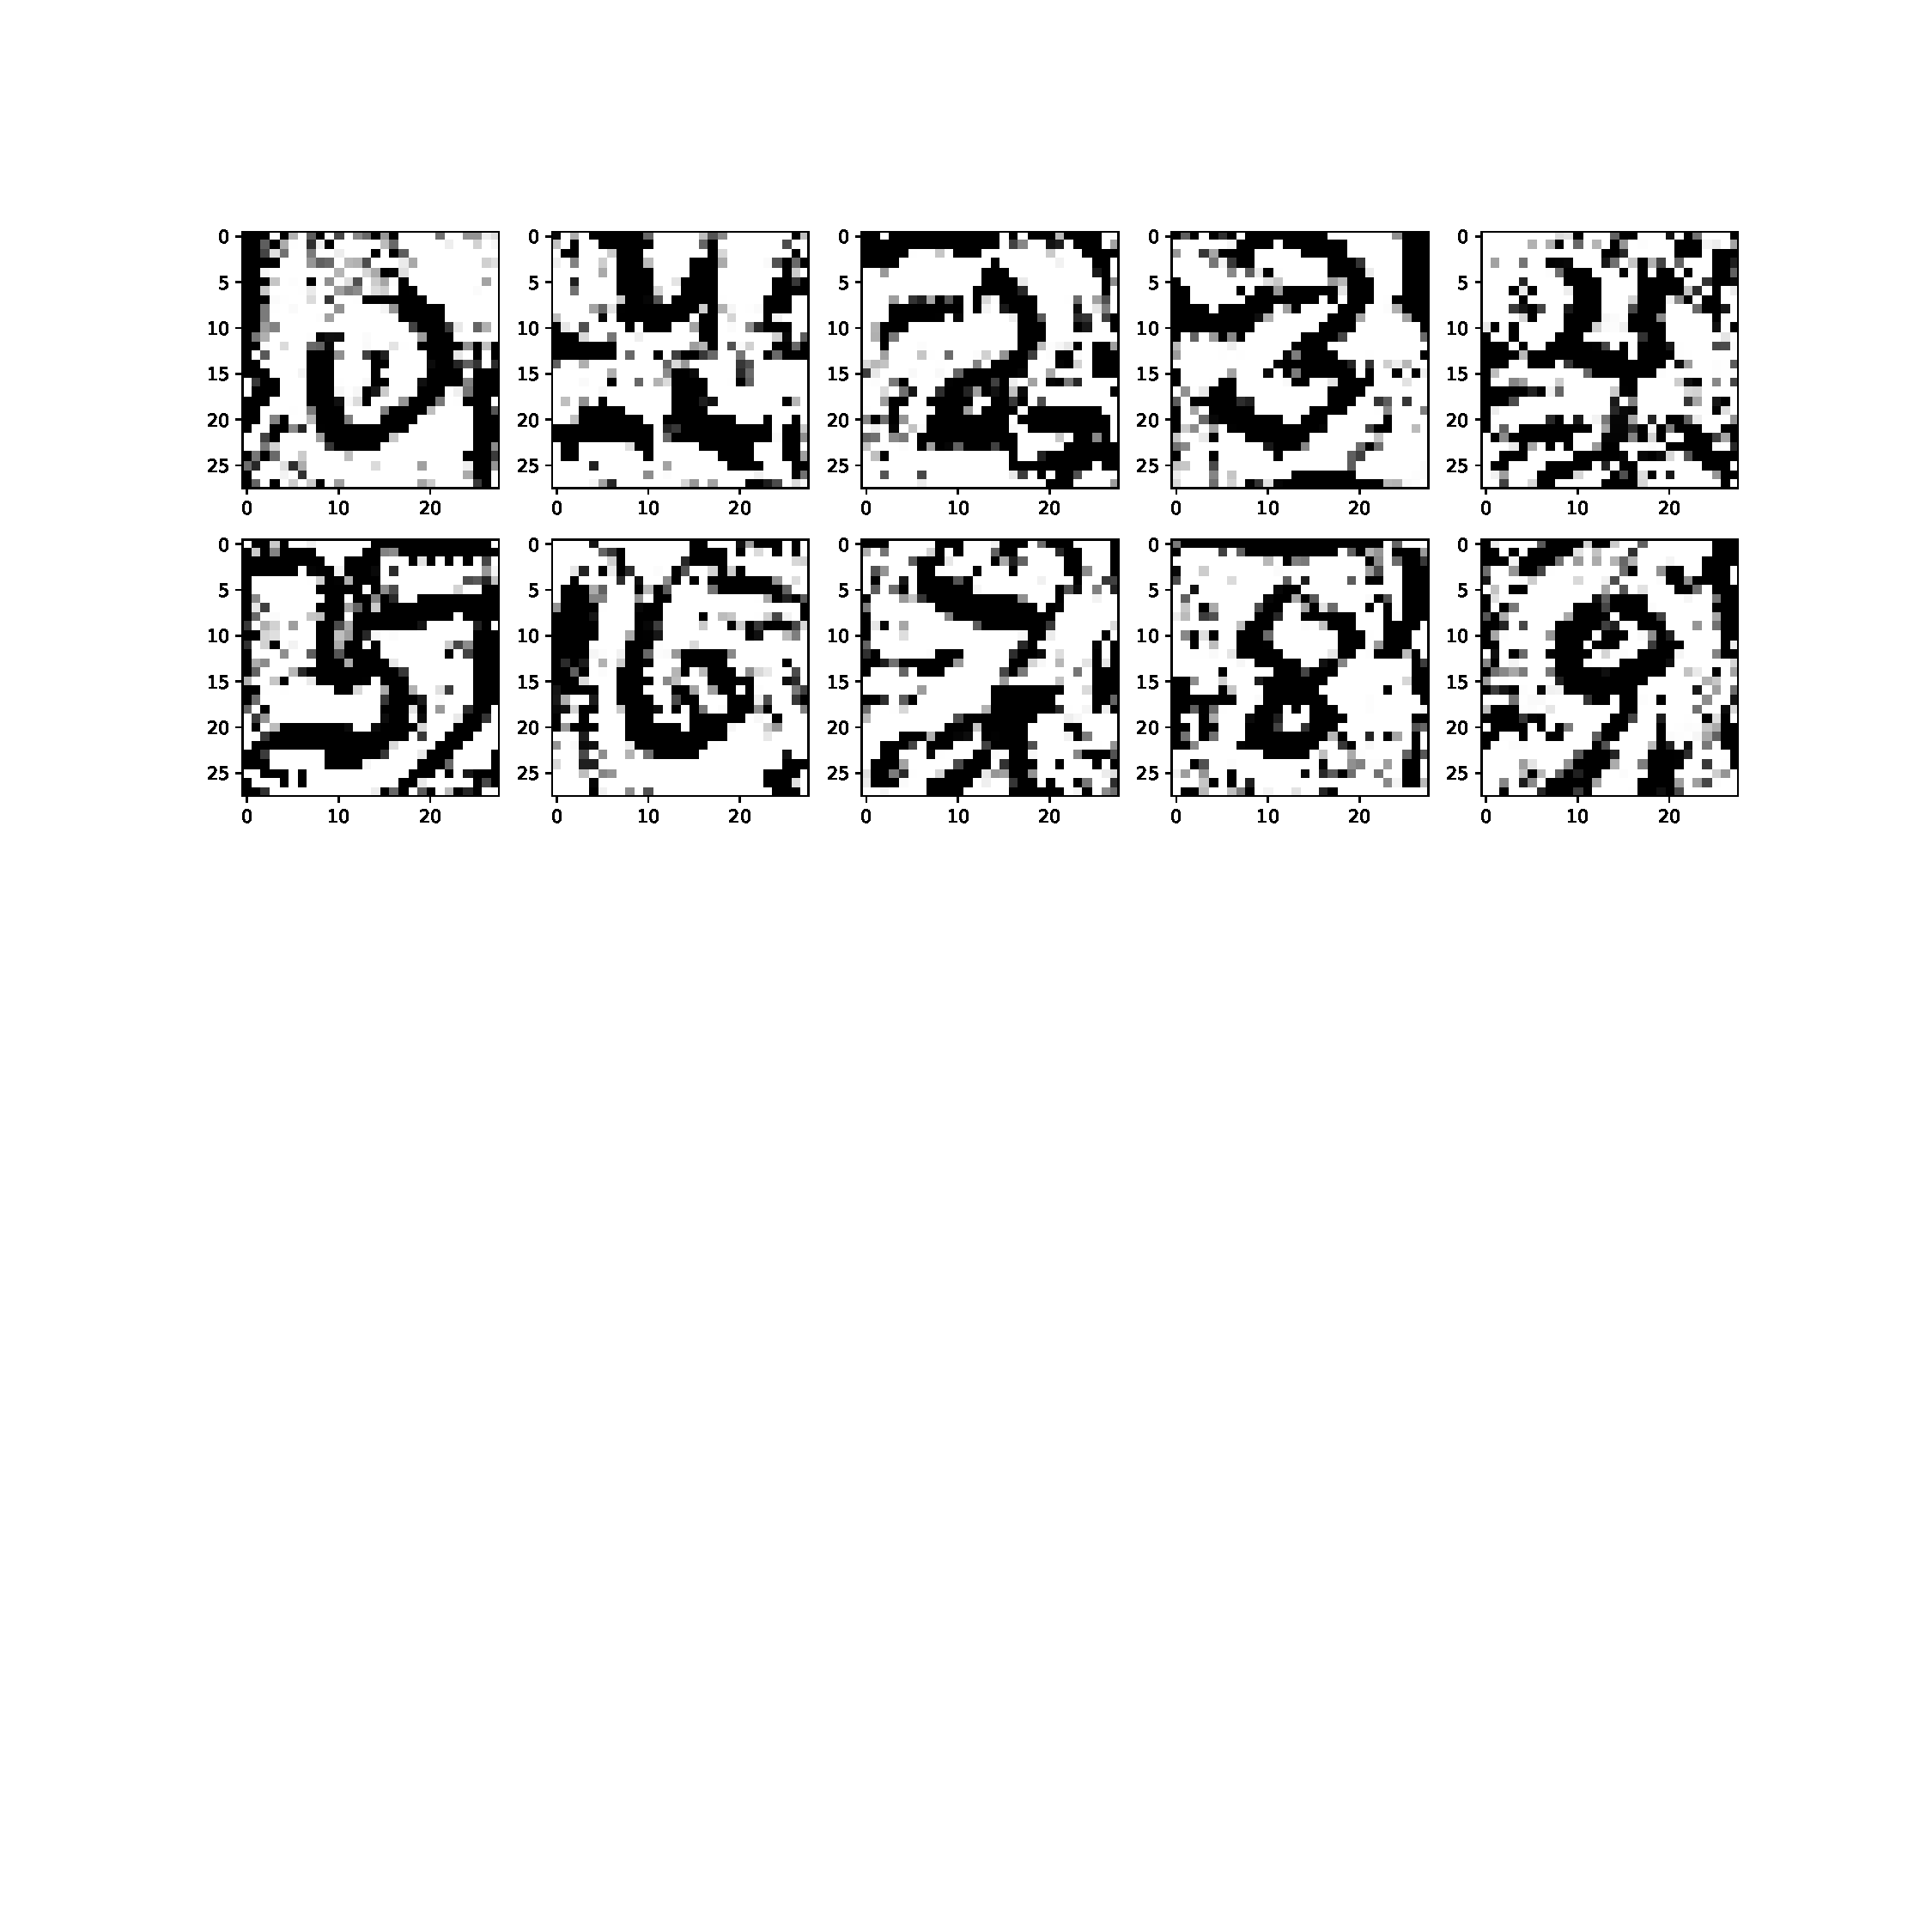
\includegraphics[width=\textwidth]{images/Native_attack/Mnistattack_native.pdf}
         \vspace{-8em}
         \caption{SPML+Native TensorFlow; and, Accuracy=99.55\%}
         \label{default}
     \end{subfigure}
     \begin{subfigure}{.325\textwidth}
         \includegraphics[width=\textwidth]{images/Native_attack/Mnistattack.2.pdf}
         \vspace{-8em}
         \caption{SPML+Privacy; $\epsilon$=0.2; and, Accuracy=10.12\%}
         \label{default}
     \end{subfigure}
     \begin{subfigure}{.325\textwidth}
         \includegraphics[width=\textwidth]{images/Native_attack/Mnistattack1.pdf}
         \vspace{-8em}
         \caption{SPML+Privacy; $\epsilon$=1 ; and, Accuracy=10.91\%}
         \label{default}
     \end{subfigure}
     \begin{subfigure}{.325\textwidth}
         \includegraphics[width=\textwidth]{images/Native_attack/Mnistattack2.pdf}
         \vspace{-8em}
         \caption{SPML+Privacy; $\epsilon$=2 ; and, Accuracy=10.63\%}
         \label{default}
     \end{subfigure}
     \begin{subfigure}{.325\textwidth}
         \includegraphics[width=\textwidth]{images/Native_attack/Mnistattack4.pdf}
         \vspace{-8em}
         \caption{SPML+Privacy; $\epsilon$=4 ; and, Accuracy=66.3\%}
         \label{default}
     \end{subfigure}
     \begin{subfigure}{.325\textwidth}
         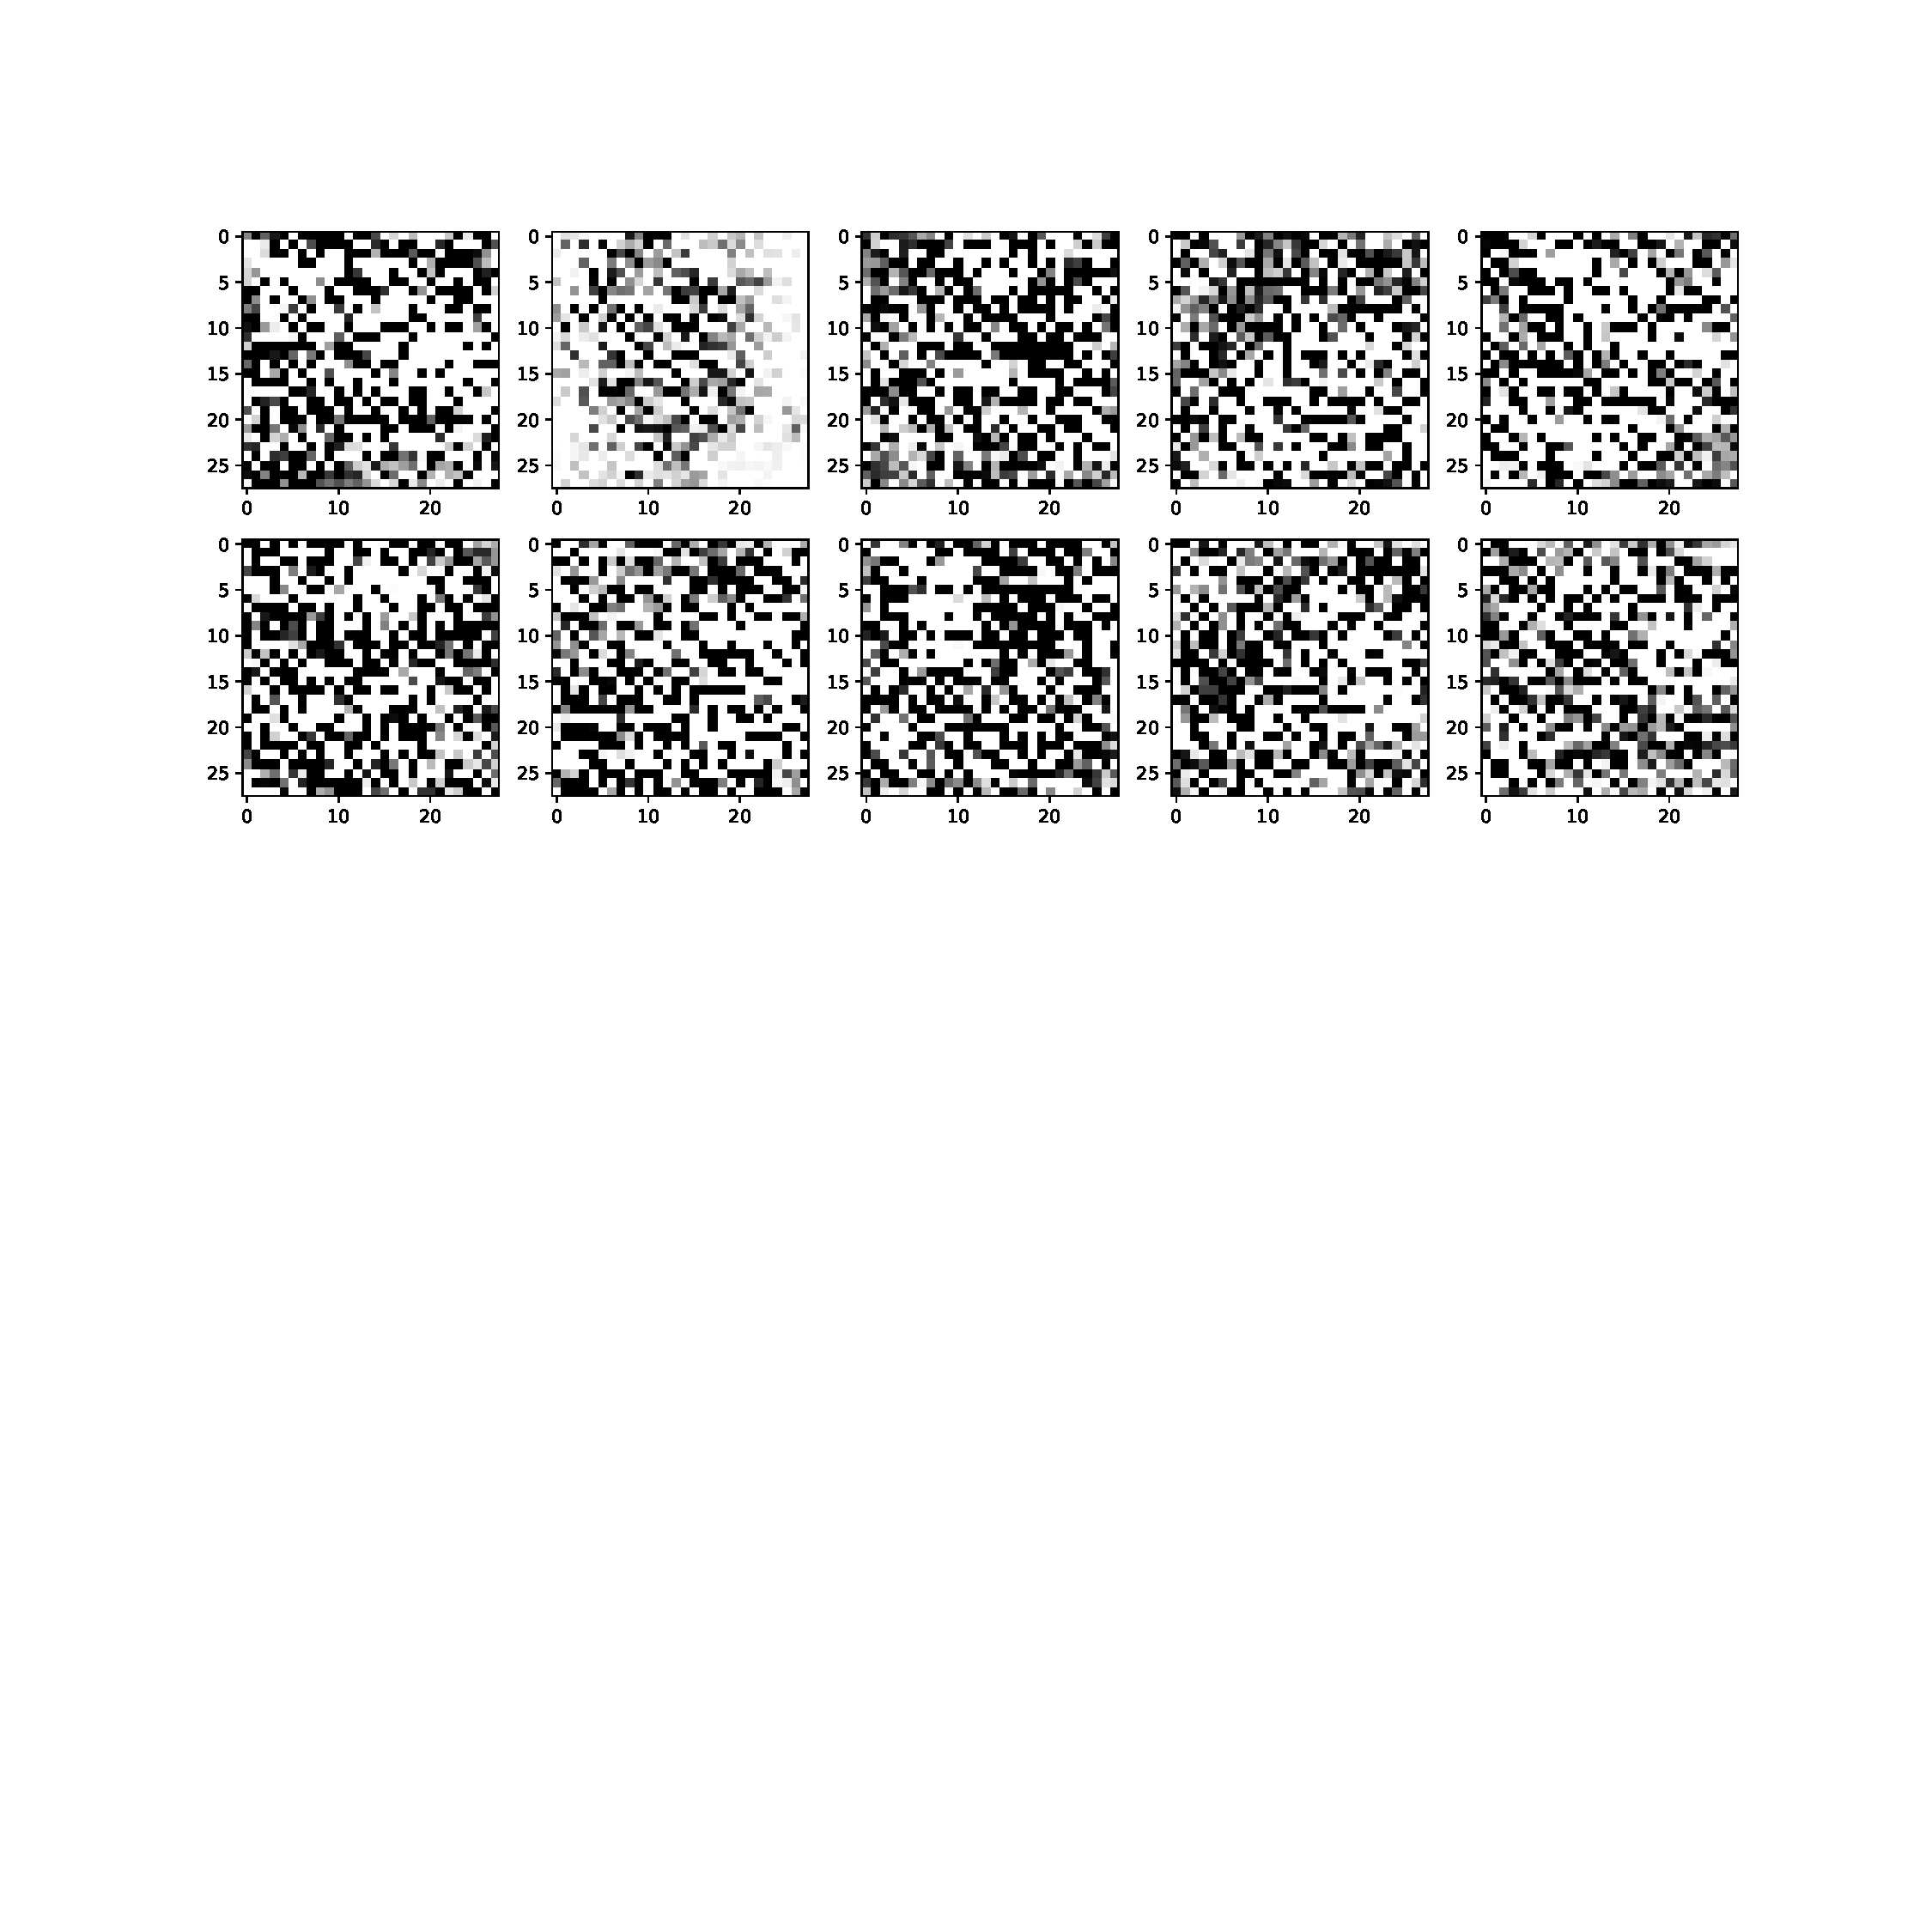
\includegraphics[width=\textwidth]{images/Native_attack/Mnistattack6.pdf}
         \vspace{-8em}
         \caption{SPML+Privacy; $\epsilon$=6 ; and, Accuracy=80.19\%}
         \label{default}
     \end{subfigure}
     \begin{subfigure}{.325\textwidth}
         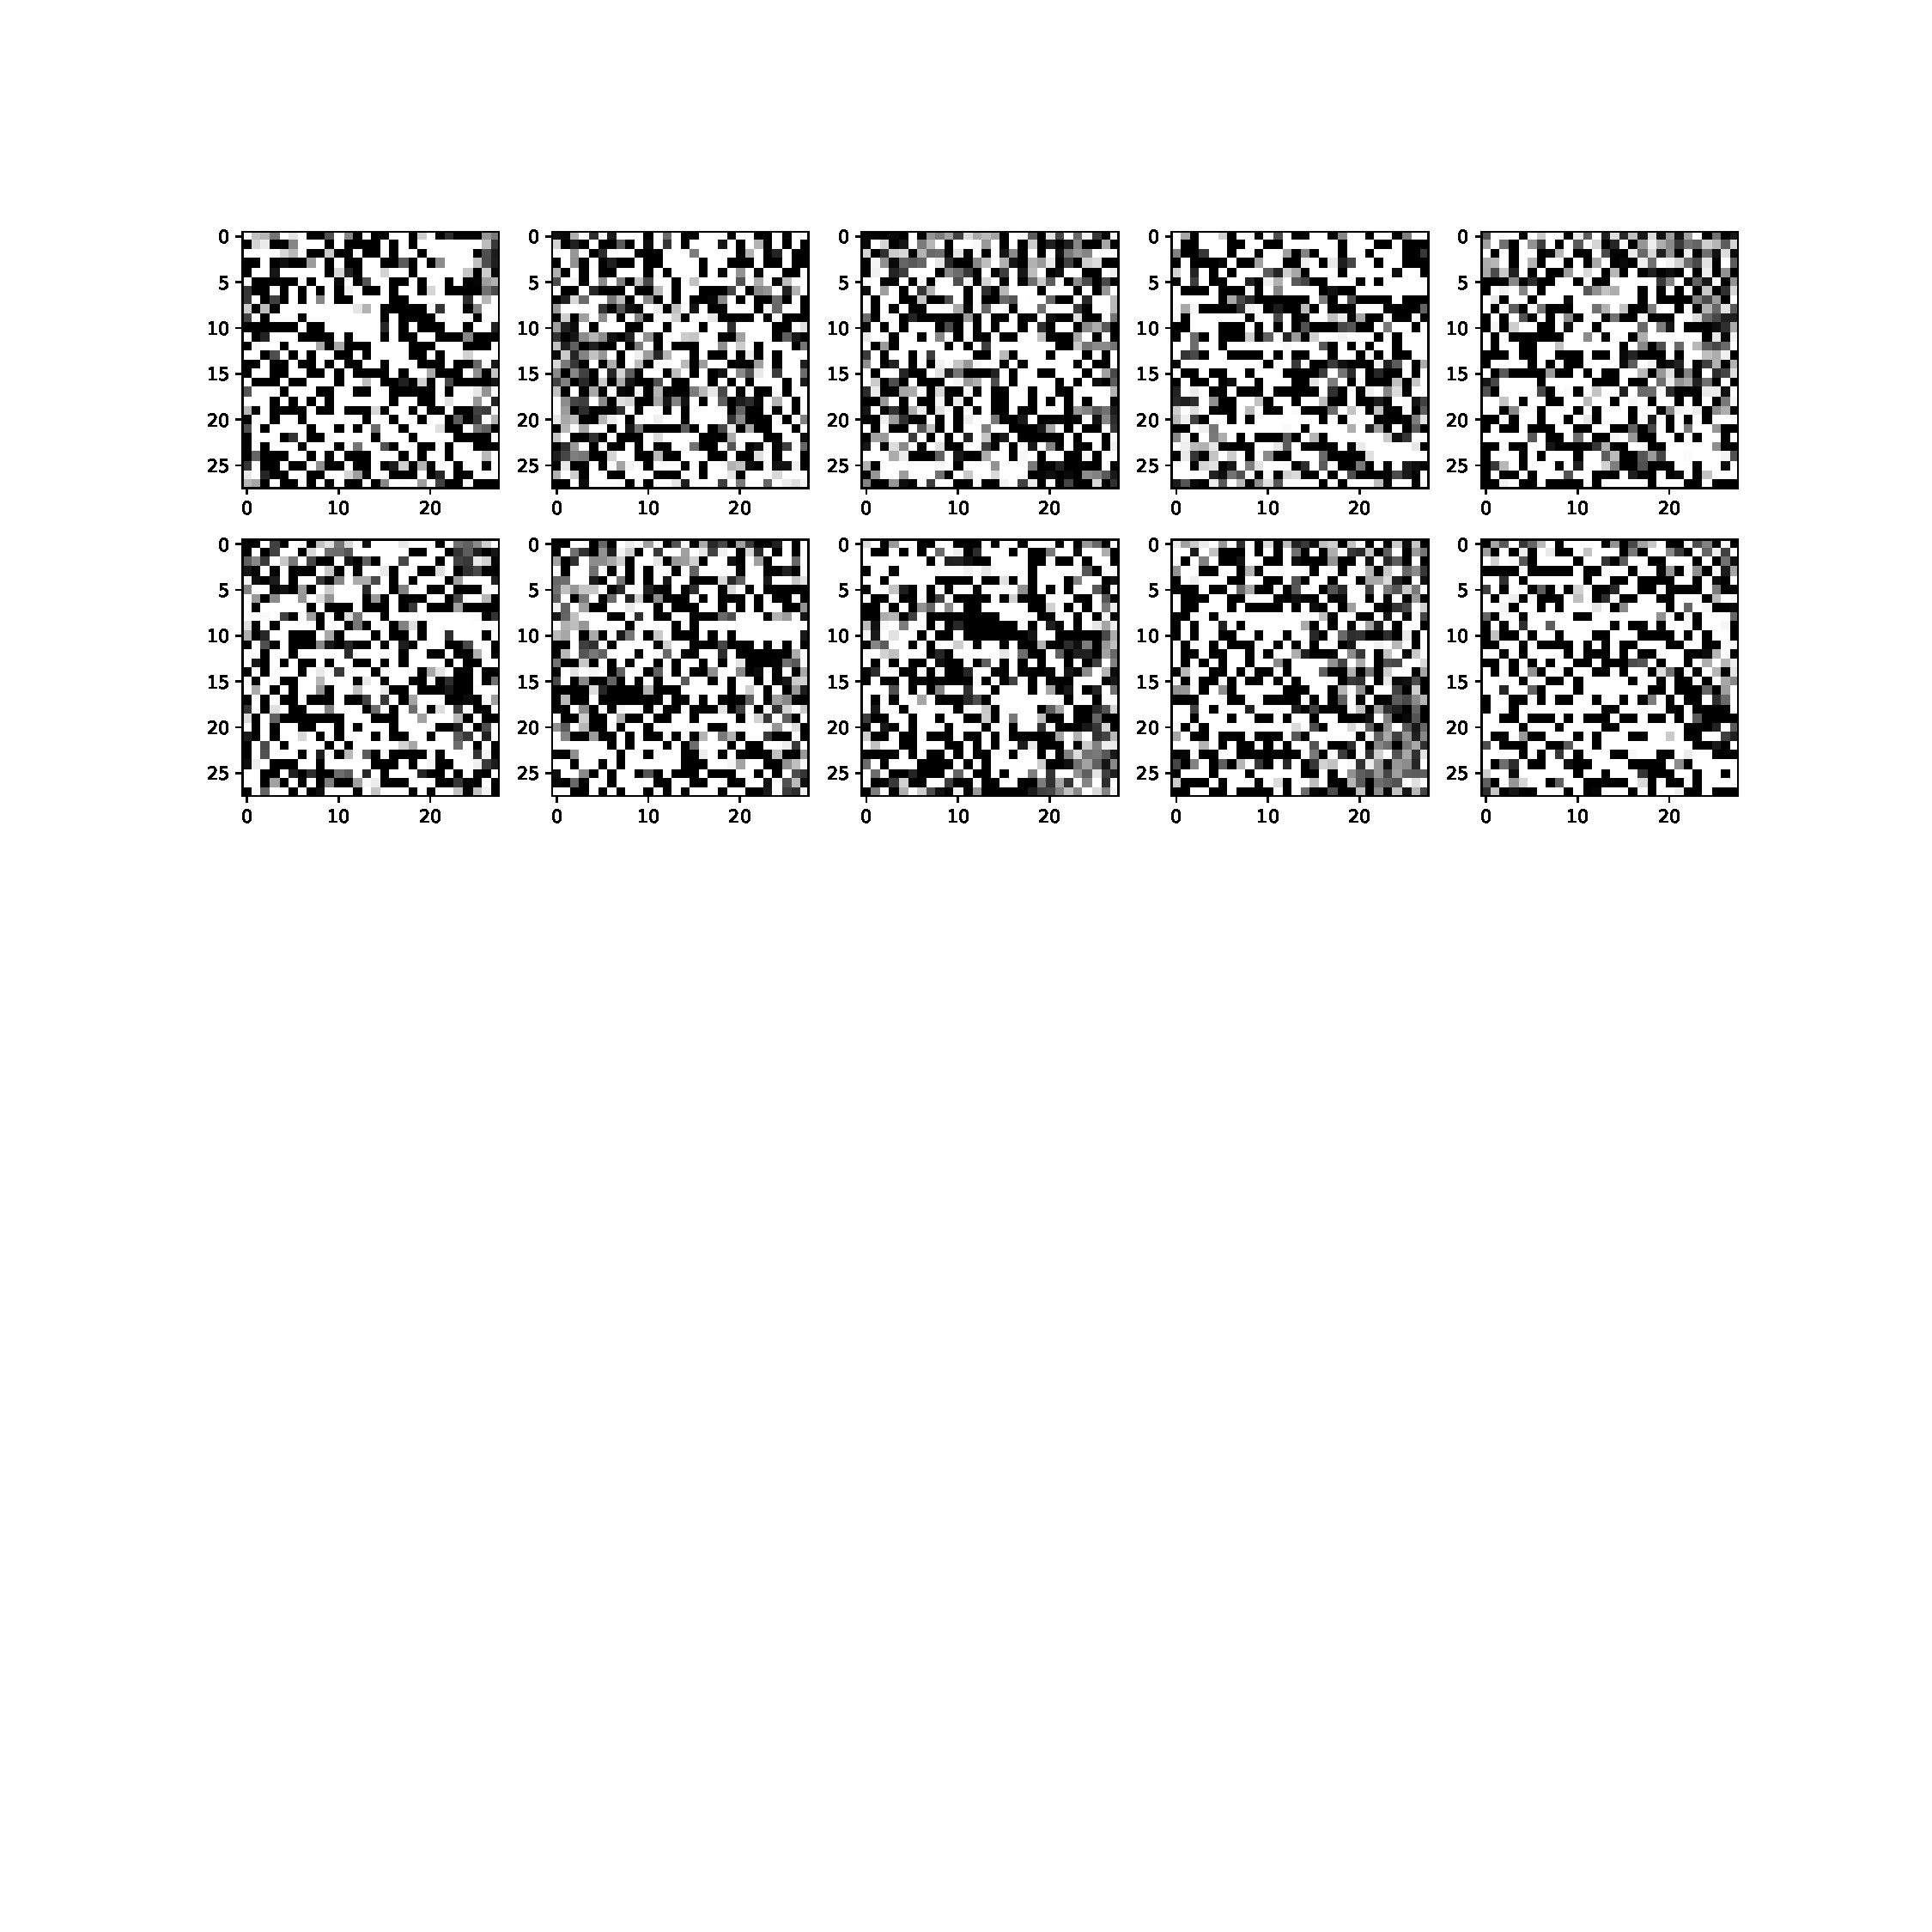
\includegraphics[width=\textwidth]{images/Native_attack/Mnistattack8.pdf}
         \vspace{-8em}
         \caption{SPML+Privacy; $\epsilon$=8 ; and, Accuracy=85.36\%}
         \label{default}
     \end{subfigure}
        \caption{Model inversion attack images - Native mode without Intel SGX and SCONE}
        \label{default}
\end{figure}

\begin{figure}
     \begin{subfigure}{.325\textwidth}
         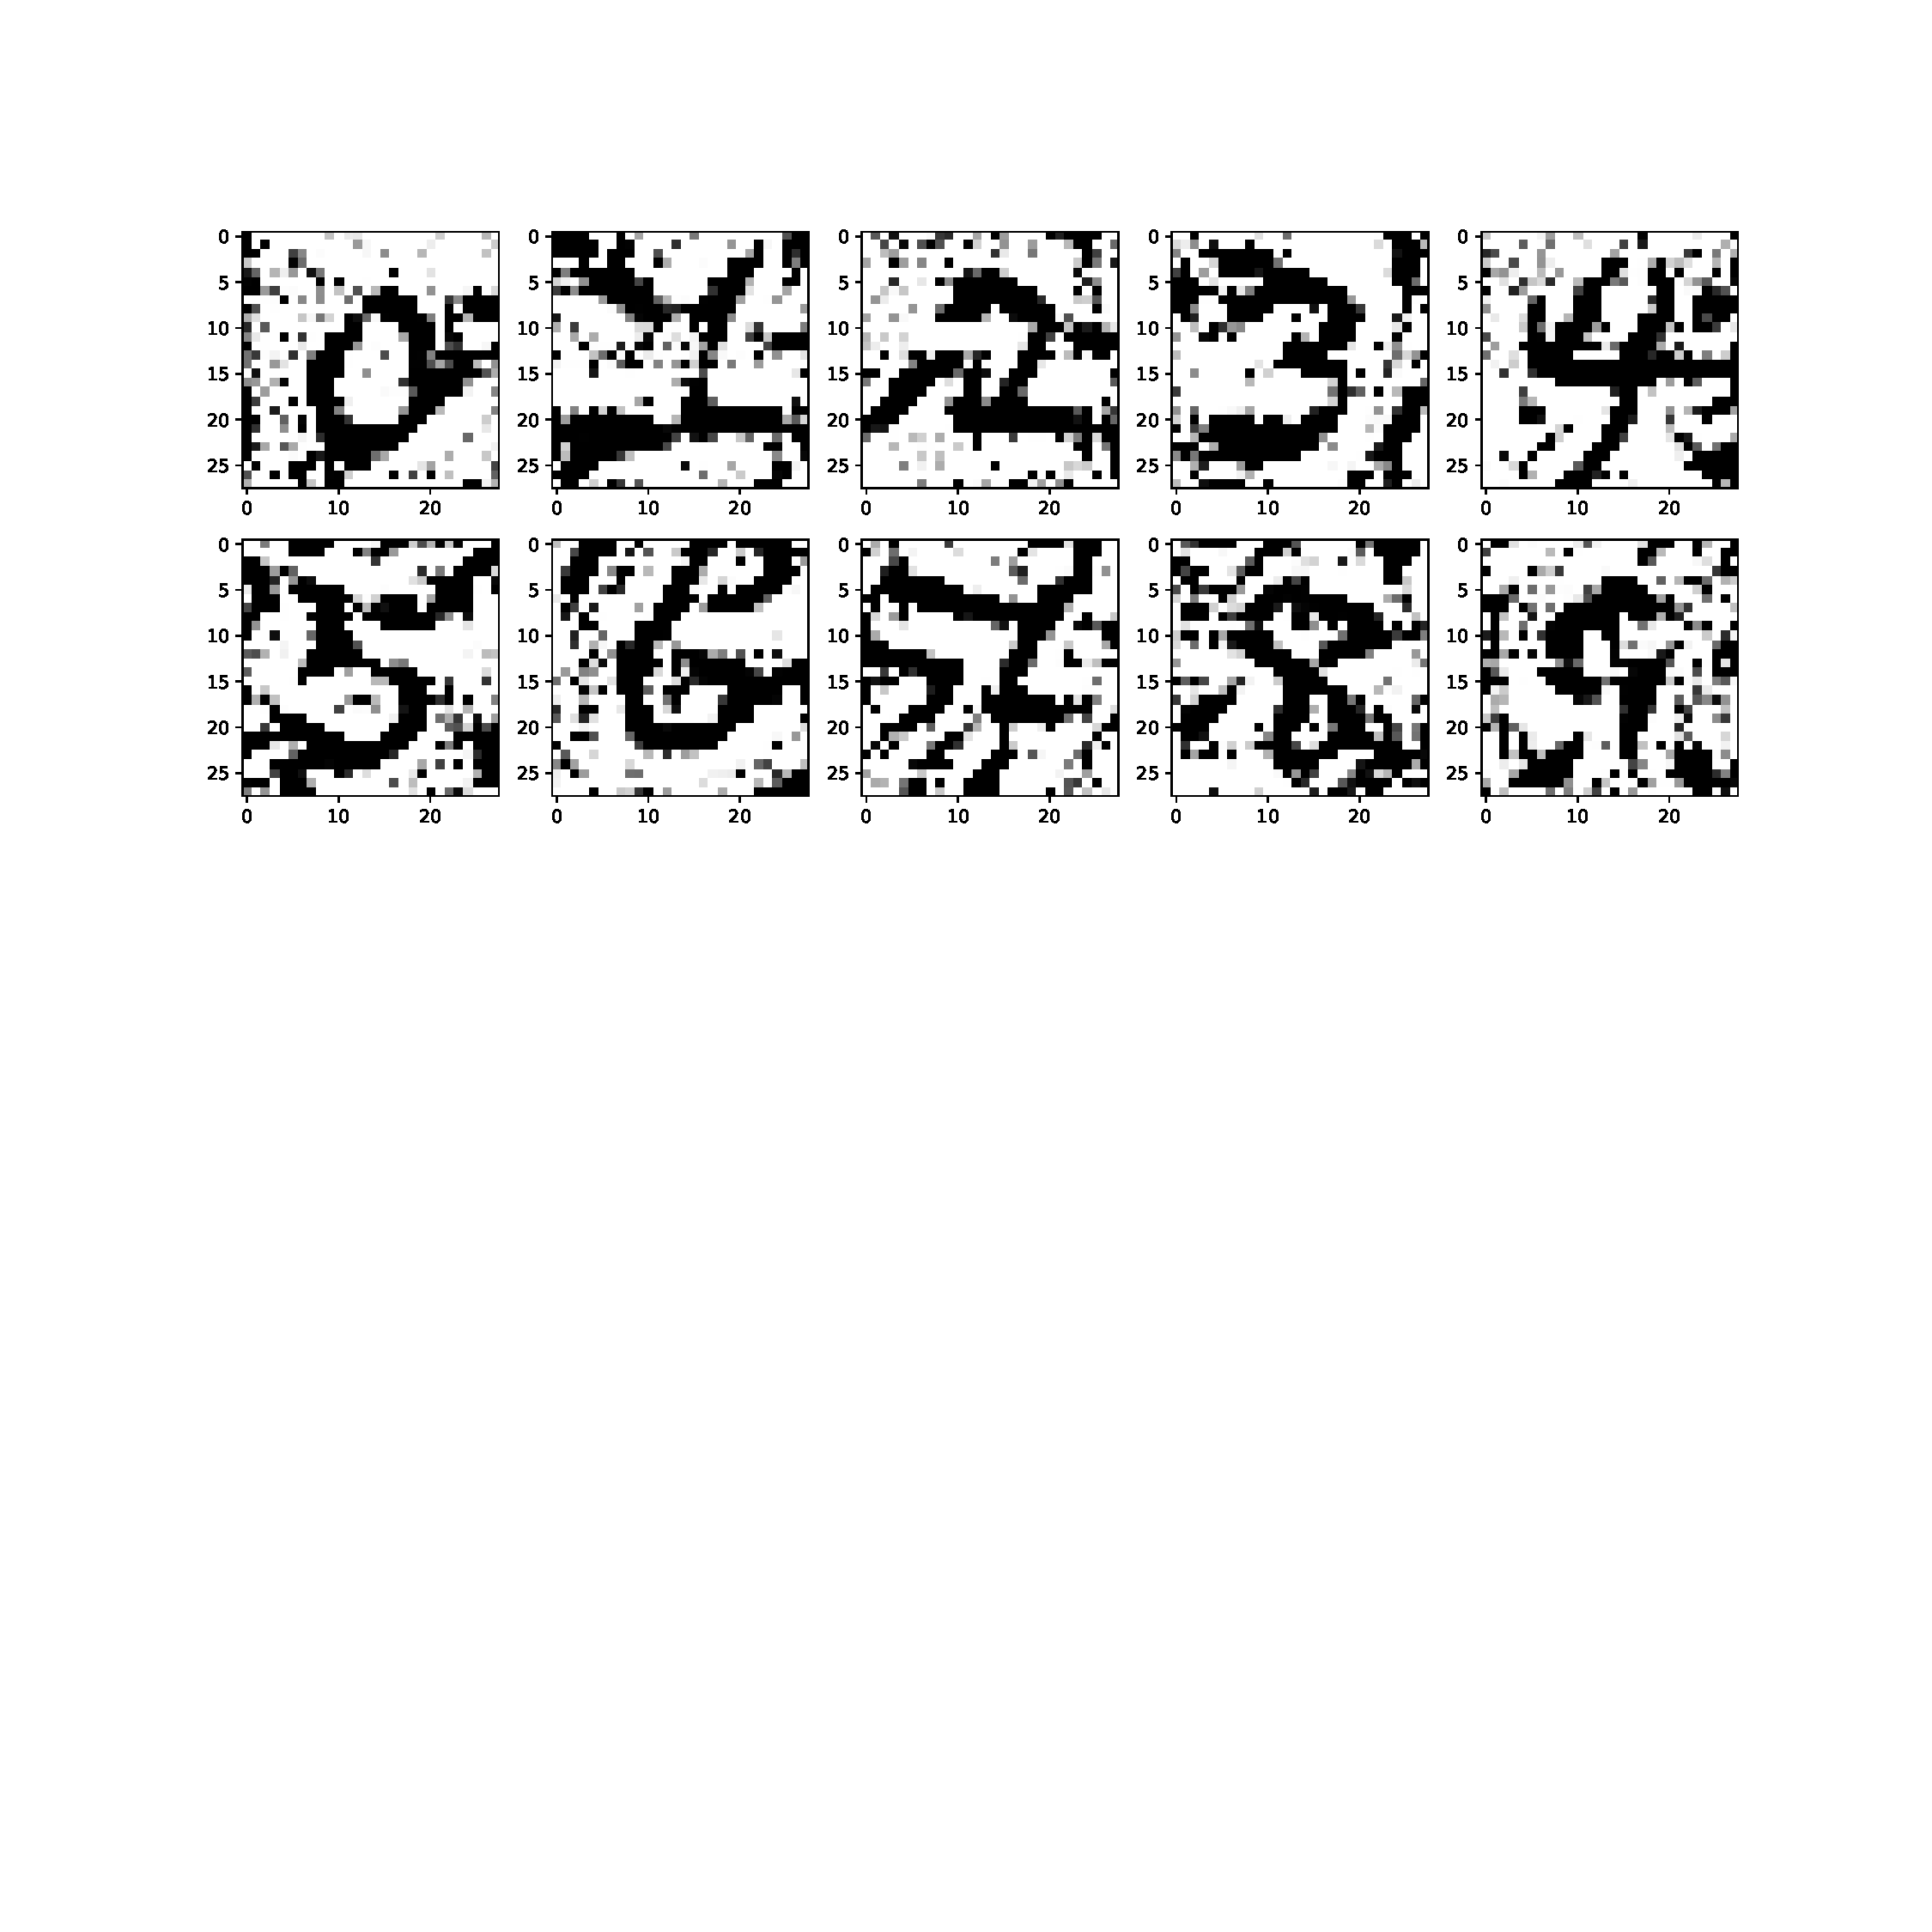
\includegraphics[width=\textwidth]{images/Sim_attack/Mnistattack_native.pdf}
         \vspace{-8em}
         \caption{SPML+Native TensorFlow; and, accuracy=99.72\%}
         \label{default}
     \end{subfigure}
     \begin{subfigure}{.325\textwidth}
         \includegraphics[width=\textwidth]{images/Sim_attack/Mnistattack.2.pdf}
         \vspace{-8em}
         \caption{SPML+Privacy; $\epsilon$=0.2; and, Accuracy=11.66\%}
         \label{default}
     \end{subfigure}
     \begin{subfigure}{.325\textwidth}
         \includegraphics[width=\textwidth]{images/Sim_attack/Mnistattack1.pdf}
         \vspace{-8em}
         \caption{SPML+Privacy; $\epsilon$=1; and, Accuracy=10.07\%}
         \label{default}
     \end{subfigure}
     \begin{subfigure}{.325\textwidth}
         \includegraphics[width=\textwidth]{images/Sim_attack/Mnistattack2.pdf}
         \vspace{-8em}
         \caption{SPML+Privacy; $\epsilon$=2; and, Accuracy=10.54\%}
         \label{default}
     \end{subfigure}
     \begin{subfigure}{.325\textwidth}
         \includegraphics[width=\textwidth]{images/Sim_attack/Mnistattack4.pdf}
         \vspace{-8em}
         \caption{SPML+Privacy; $\epsilon$=4; and, Accuracy=67.76\%}
         \label{default}
     \end{subfigure}
     \begin{subfigure}{.325\textwidth}
         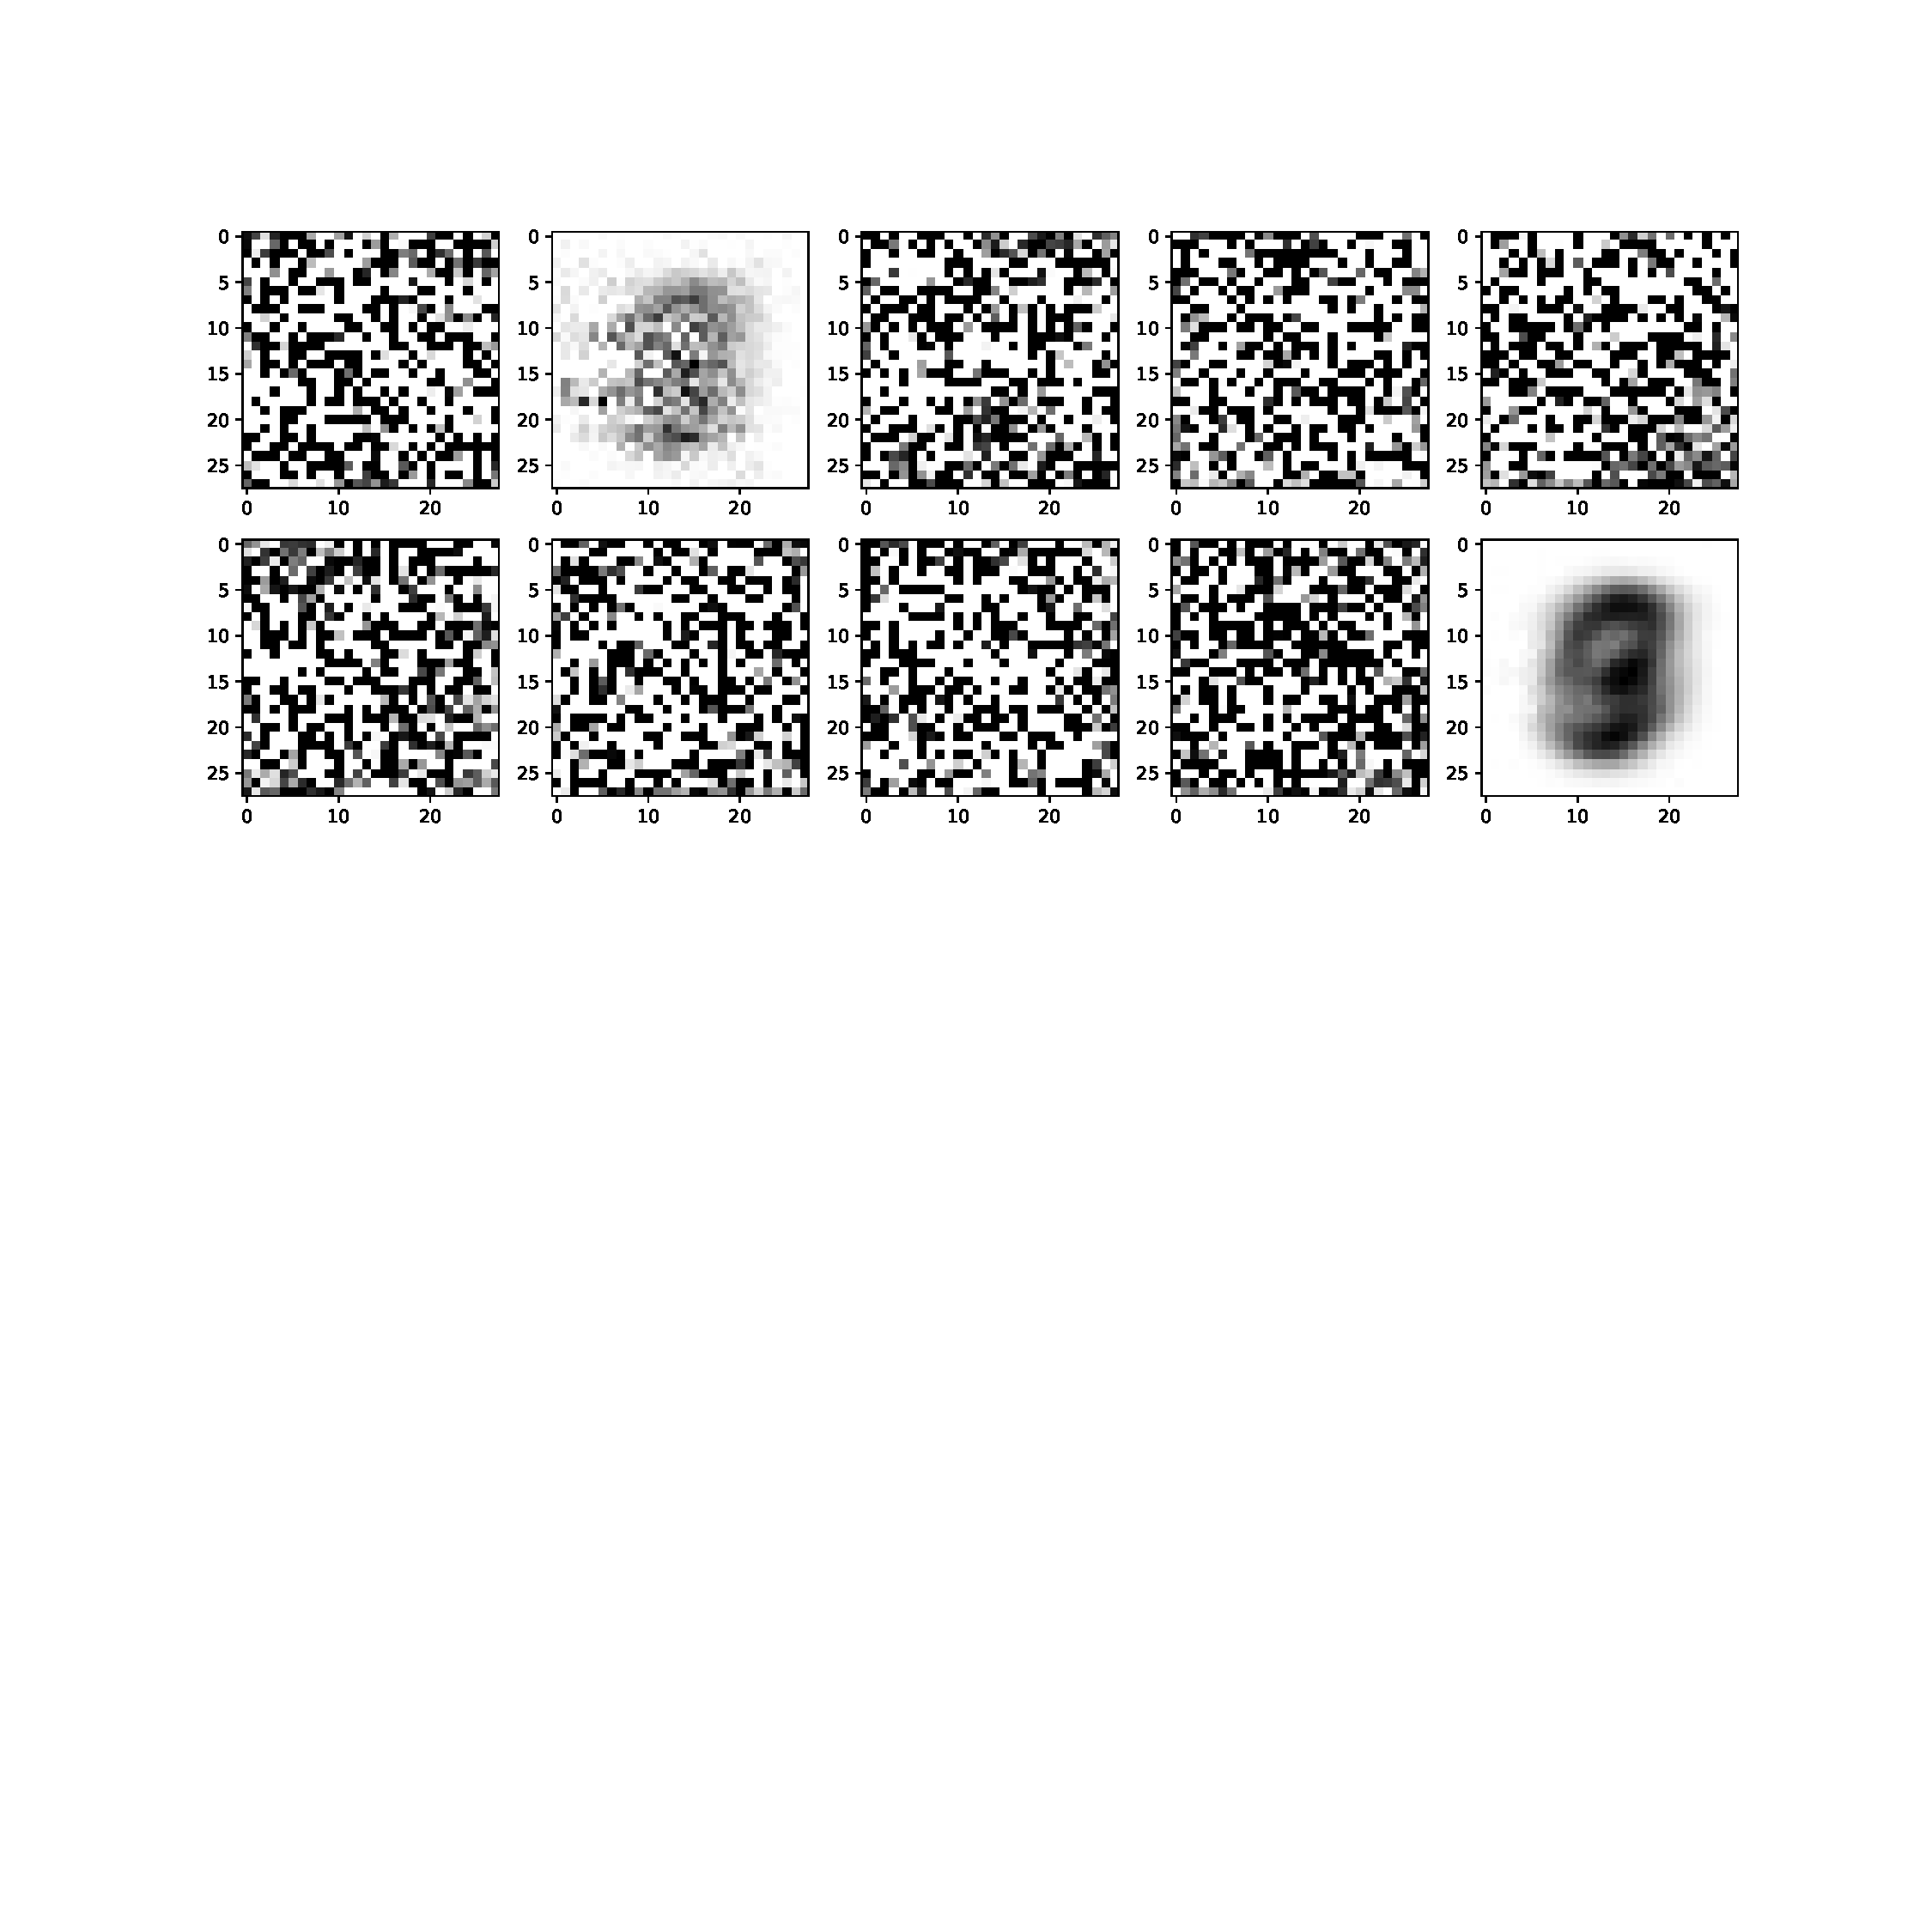
\includegraphics[width=\textwidth]{images/Sim_attack/Mnistattack6.pdf}
         \vspace{-8em}
         \caption{SPML+Privacy; $\epsilon$=6; and, Accuracy=71.6\%}
         \label{default}
     \end{subfigure}
     \begin{subfigure}{.325\textwidth}
         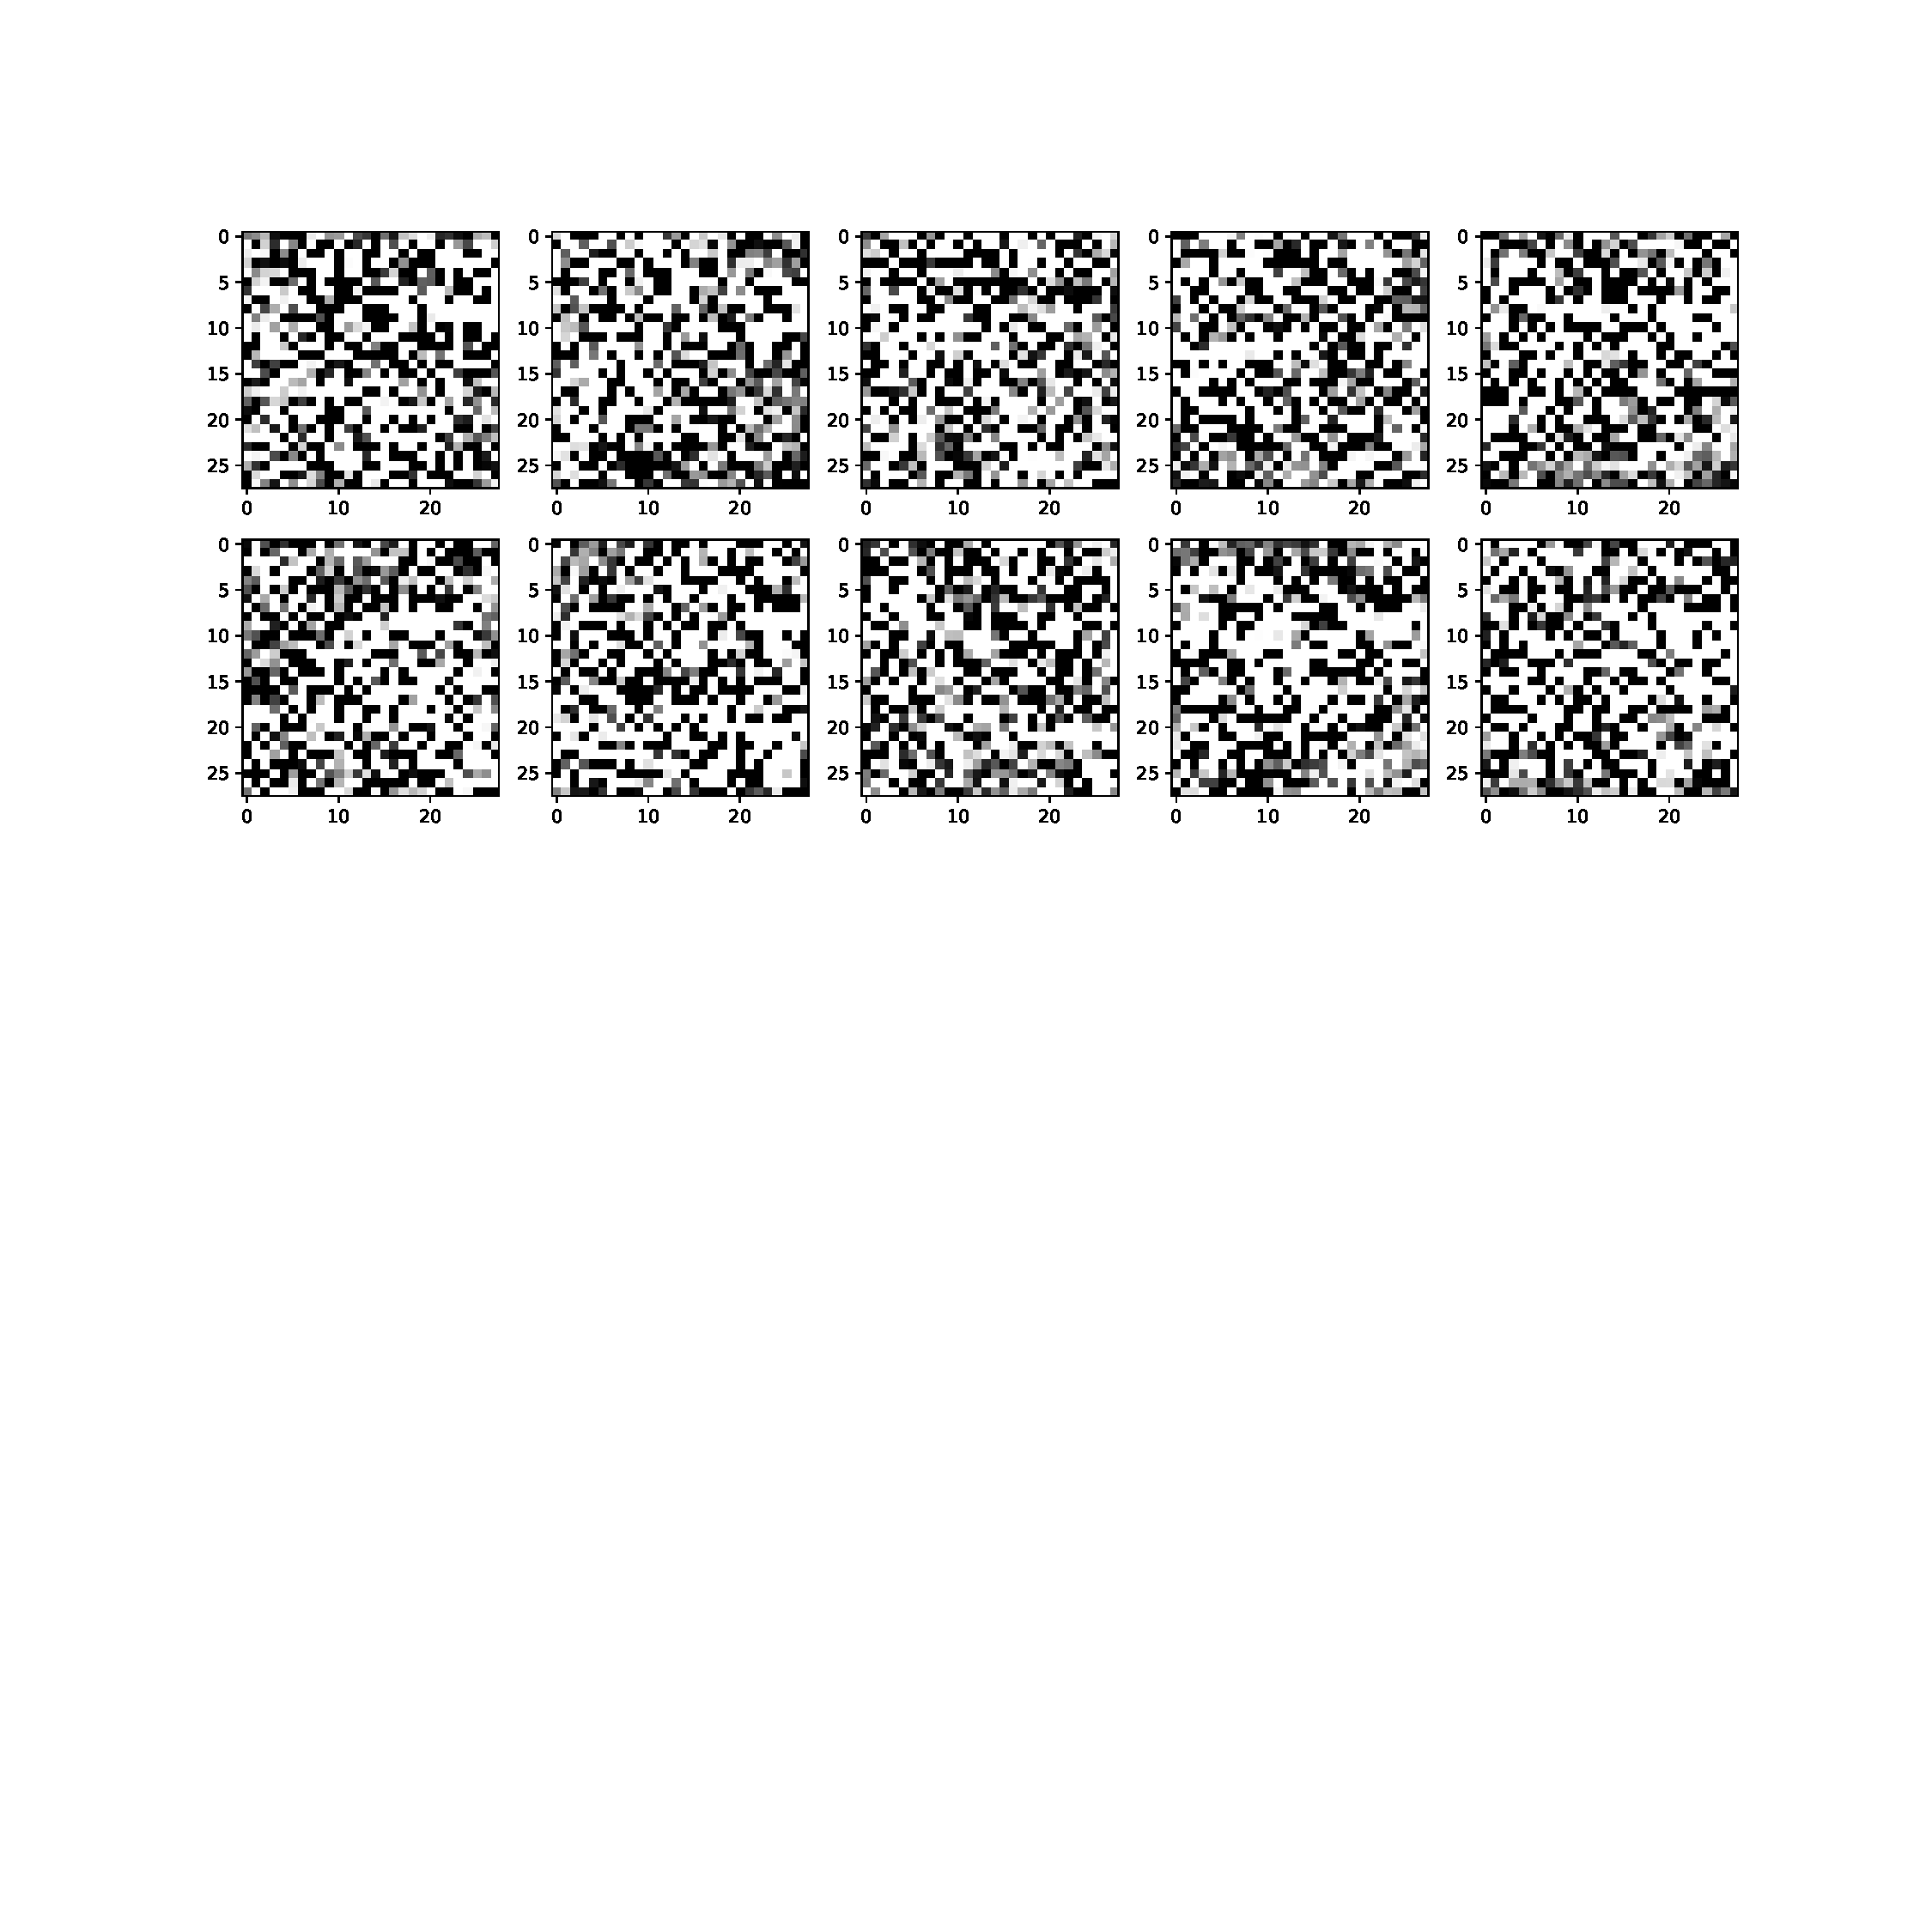
\includegraphics[width=\textwidth]{images/Sim_attack/Mnistattack8.pdf}
         \vspace{-8em}
         \caption{SPML+Privacy; $\epsilon$=8; and, Accuracy=84.37\%}
         \label{default}
     \end{subfigure}
        \caption{Model inversion attack images - SCONE simulation mode without Intel SGX and with SCONE}
        \label{default}
\end{figure}

\begin{figure}
     \begin{subfigure}{.325\textwidth}
         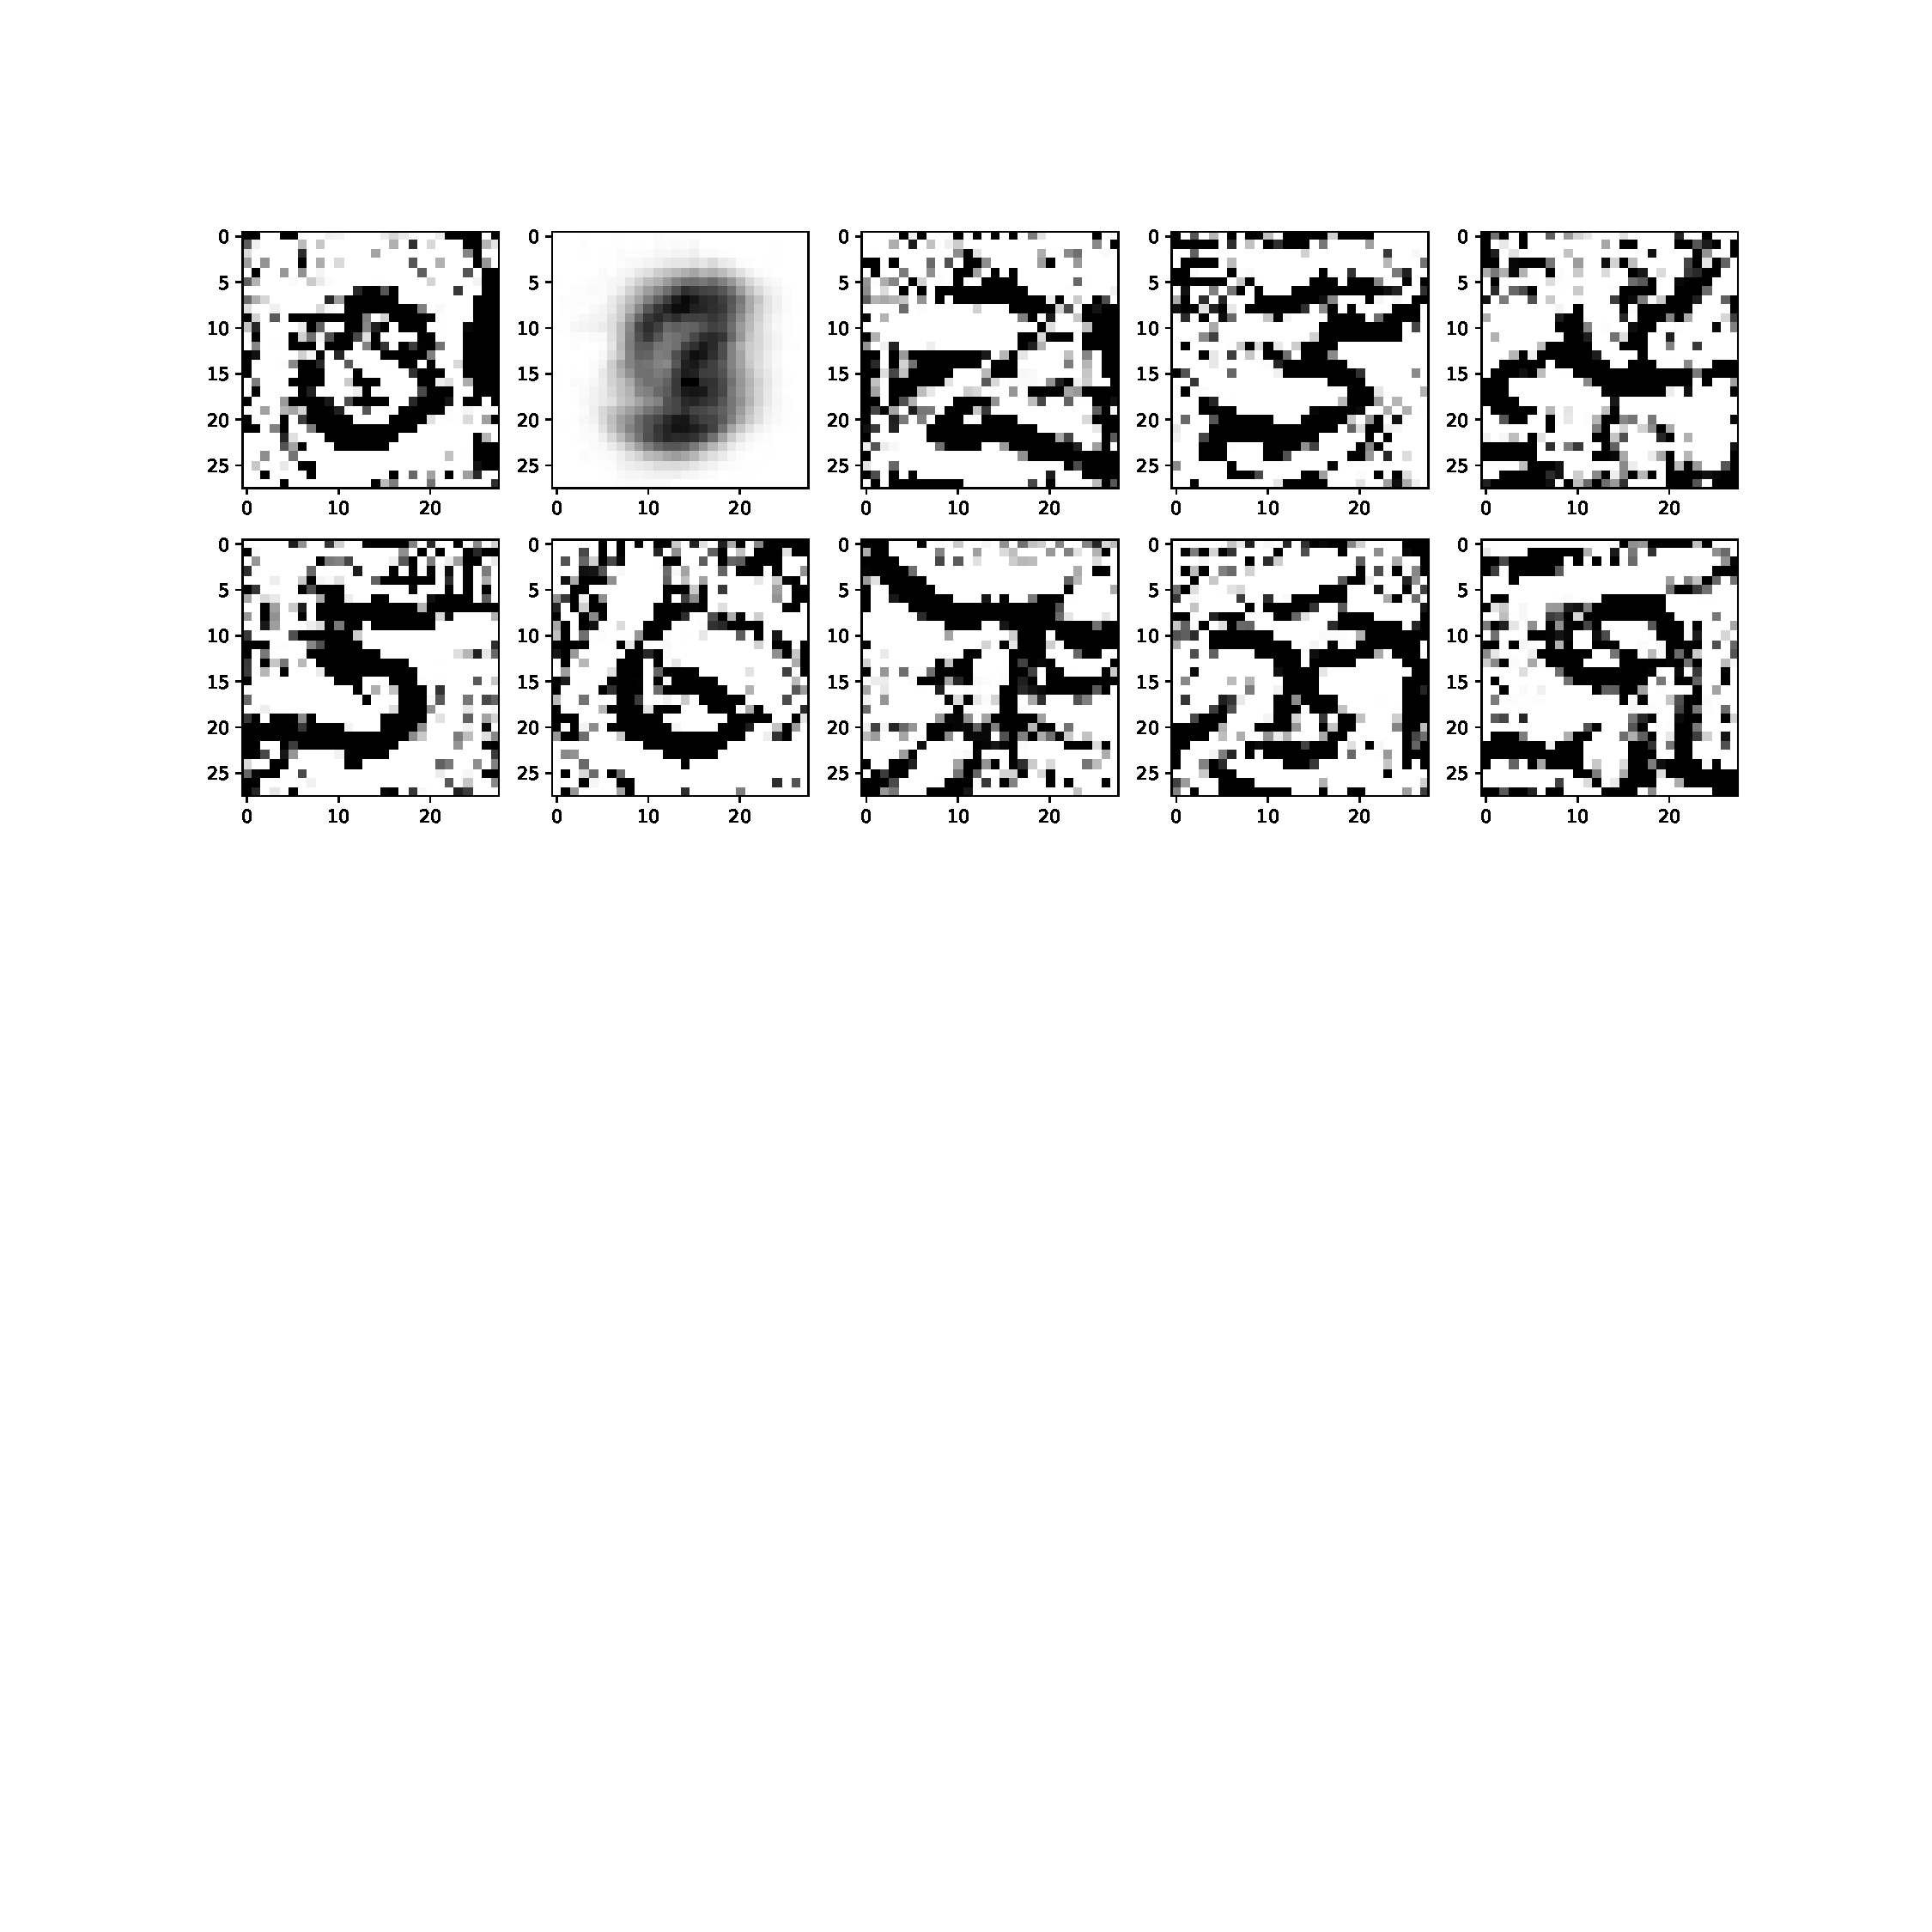
\includegraphics[width=\textwidth]{images/Hw_attack/Mnistattack_native.pdf}
         \vspace{-8em}
         \caption{SPML+Native TensorFlow; and, accuracy=99.65\%}
         \label{default}
     \end{subfigure}
     \begin{subfigure}{.325\textwidth}
         \includegraphics[width=\textwidth]{images/Hw_attack/Mnistattack.2.pdf}
         \vspace{-8em}
         \caption{SPML+Privacy; $\epsilon$=0.2; and, Accuracy=10.19\%}
         \label{default}
     \end{subfigure}
     \begin{subfigure}{.325\textwidth}
         \includegraphics[width=\textwidth]{images/Hw_attack/Mnistattack1.pdf}
         \vspace{-8em}
         \caption{SPML+Privacy; $\epsilon$=1; and, Accuracy=10.13\%}
         \label{default}
     \end{subfigure}
     \begin{subfigure}{.325\textwidth}
         \includegraphics[width=\textwidth]{images/Hw_attack/Mnistattack2.pdf}
         \vspace{-8em}
         \caption{SPML+Privacy; $\epsilon$=2; and, Accuracy=10.39\%}
         \label{default}
     \end{subfigure}
     \begin{subfigure}{.325\textwidth}
         \includegraphics[width=\textwidth]{images/Hw_attack/Mnistattack4.pdf}
         \vspace{-8em}
         \caption{SPML+Privacy; $\epsilon$=4; and, Accuracy=53.13\%}
         \label{default}
     \end{subfigure}
     \begin{subfigure}{.325\textwidth}
         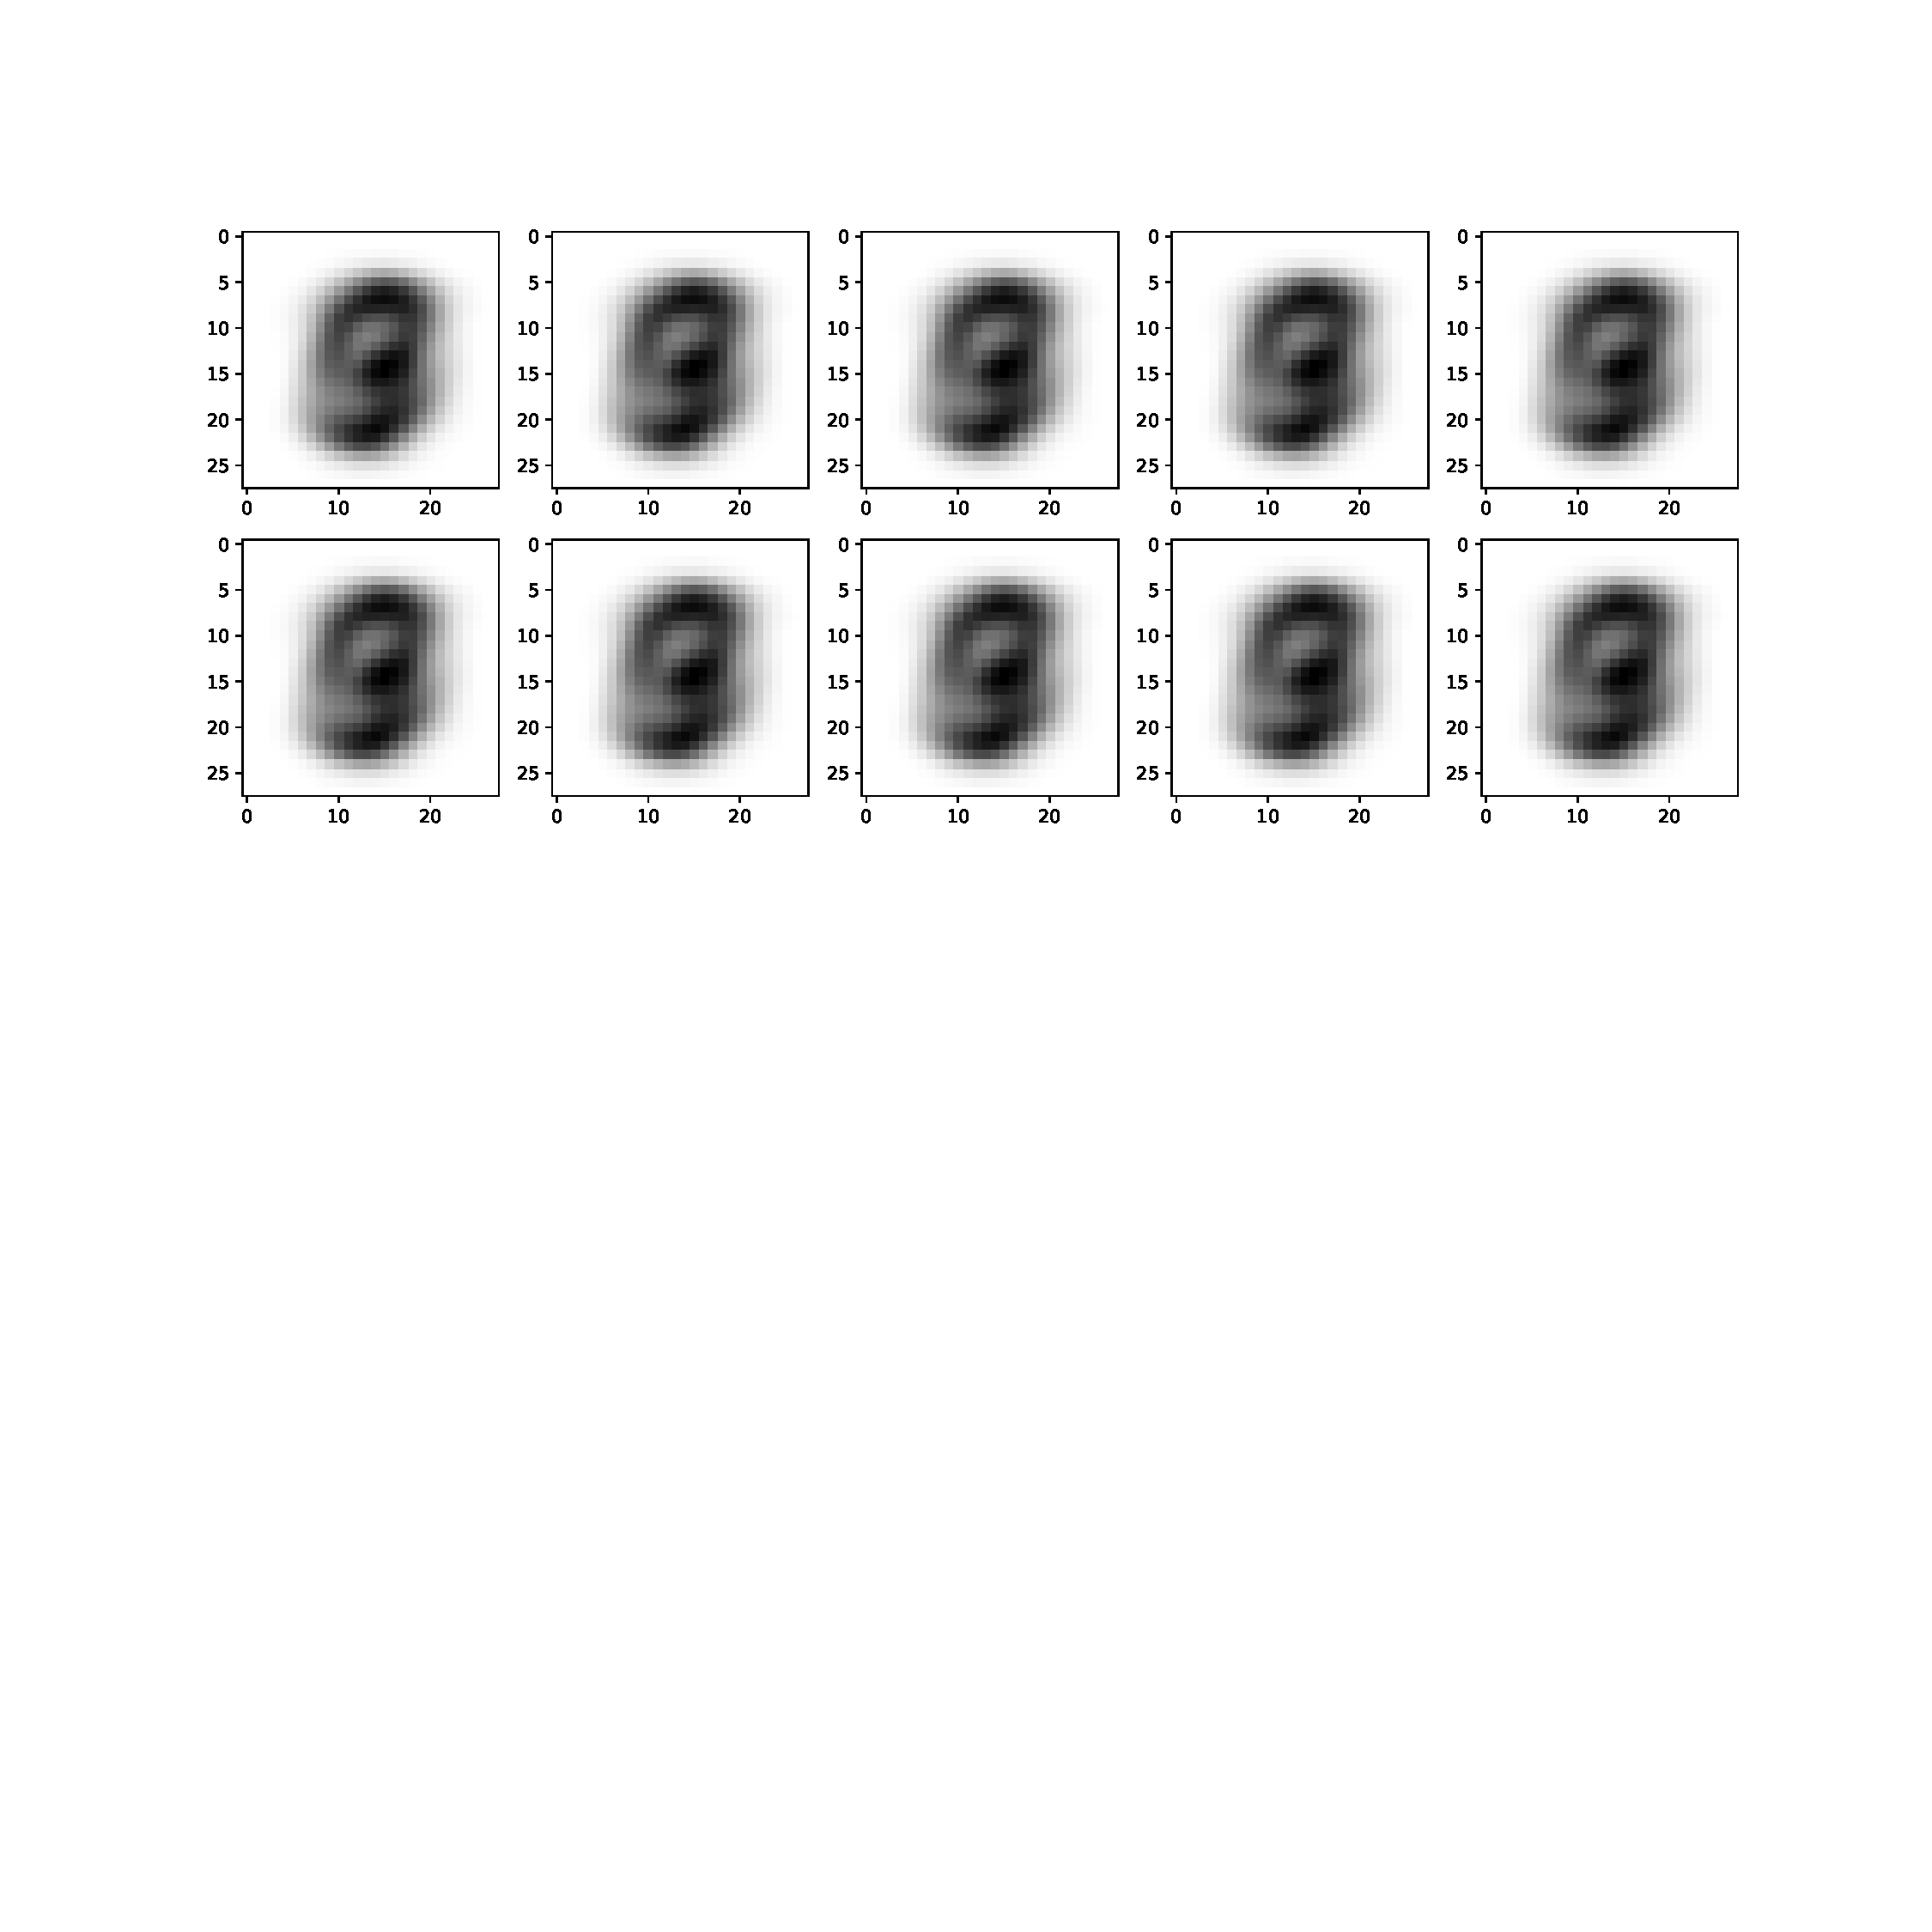
\includegraphics[width=\textwidth]{images/Hw_attack/Mnistattack6.pdf}
         \vspace{-8em}
         \caption{SPML+Privacy; $\epsilon$=6; and, Accuracy=75.92\%}
         \label{default}
     \end{subfigure}
     \begin{subfigure}{.325\textwidth}
         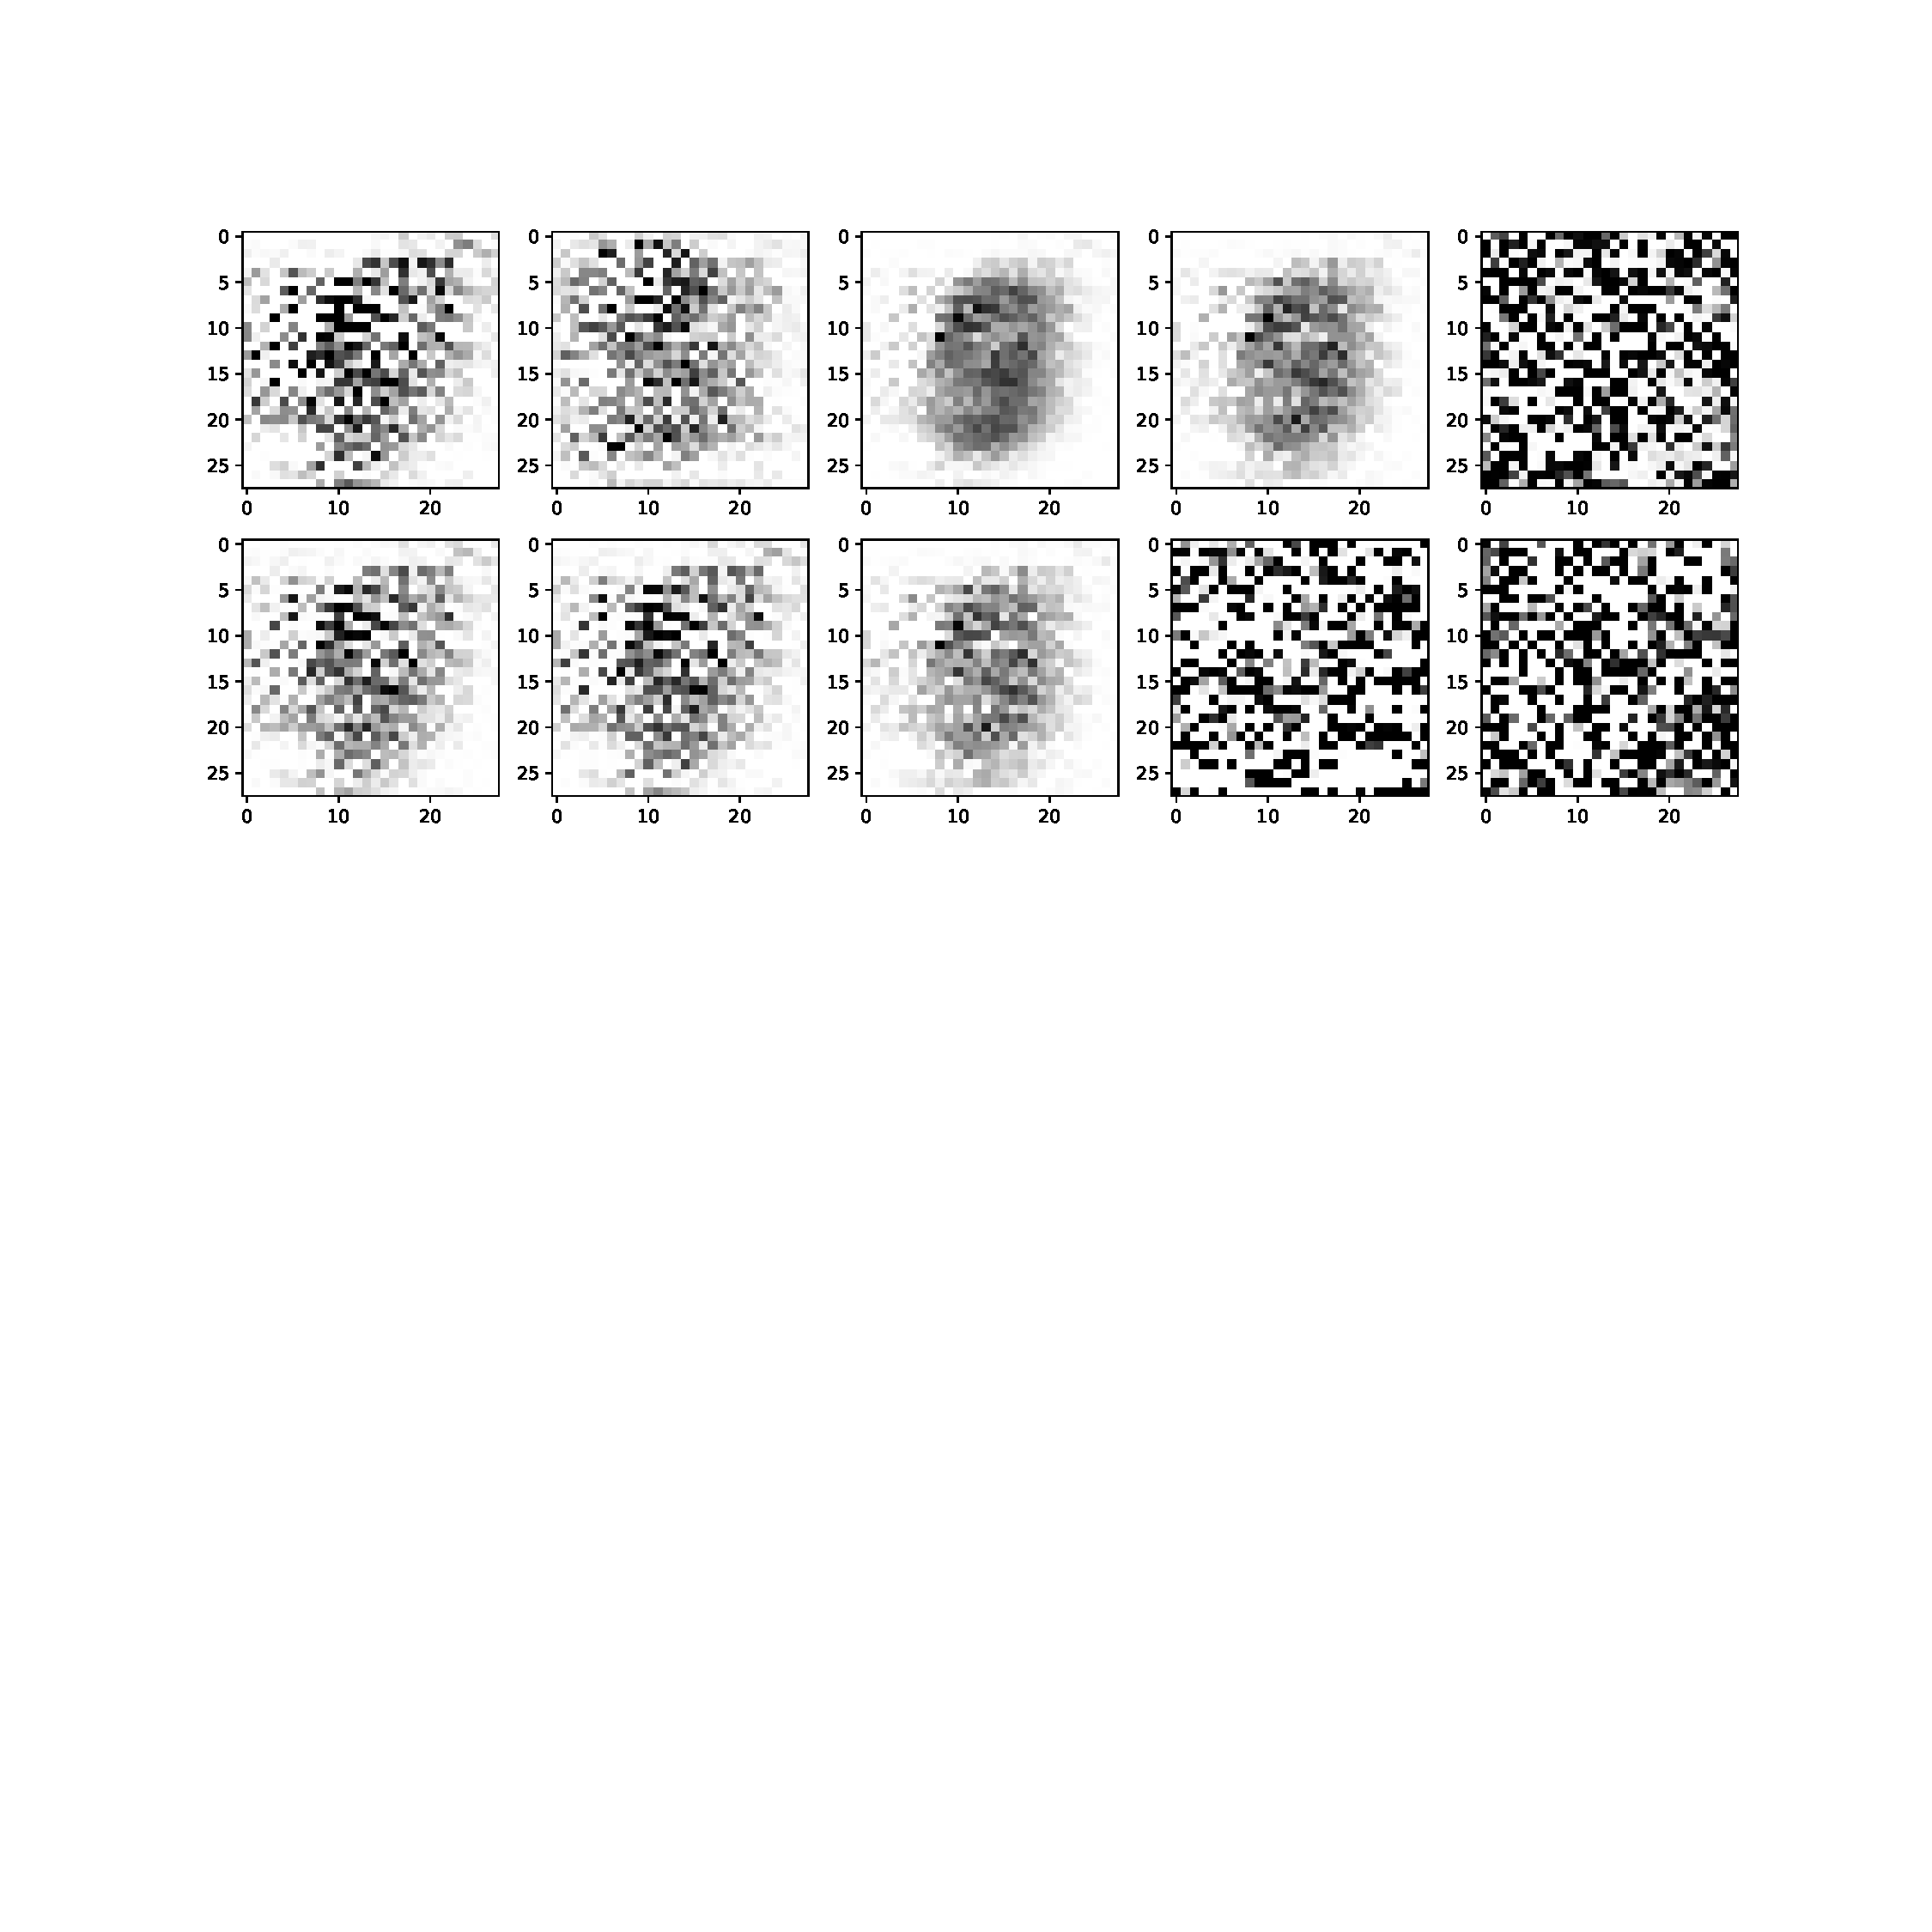
\includegraphics[width=\textwidth]{images/Hw_attack/Mnistattack8.pdf}
         \vspace{-8em}
         \caption{SPML+Privacy; $\epsilon$=8; and, Accuracy=85.93\%}
         \label{default}
     \end{subfigure}
        \caption{Model inversion attack images - SCONE hardware mode with Intel SGX and with SCONE}
        \label{default}
\end{figure}
% \addchap{Glossary}
%\appendix
% makeglossaries diplom
%\printglossary[style=altlist]
%\printglossary[type=\acronymtype,style=long]
%\markboth{}{}
%\chapter*{References}
%\addcontentsline{toc}{chapter}{References}


\chapter{Conclusion}
\label{sec:conclusion}
In this thesis, we have created a secure privacy-preserving machine learning framework SPML that enforces privacy, confidentiality, and integrity on any native machine/deep learning system. We have developed this framework with the help of Google TensorFlow \cite{24}, differential privacy library to achieve privacy \cite{11}, Intel SGX \cite{9} to achieve security goals of confidentiality and integrity and SCONE \cite{22} for integration with TEEs.

We have used the SCONE platform to achieve confidential computing using Intel SGX. SCONE give us the transparency and hides the complexities of using Intel SGX SDK. It has saved a lot of our effort which is required to integrate any existing native machine learning application with Intel SGX.

In the evaluation chapter ~\ref{sec:eval}, we have run some measurements on the popular public dataset MNIST \cite{12}, CIFAR10 \cite{13} and randomized response to get the performance overview of our system SPML. To conclude, we have divided the chapter further into two sections: (1) Effect of noise (2) Effect of randomized noise and later we have compared both of these techniques for pros and cons.

\section{Effect of noise}
The noise can be Gaussian noise or Laplace noise. We have implemented SPML with Gaussian noise. To conclude the effect of noise we will be discussing what happens when we enable (1) only privacy property (2) only security property (3) both the properties for training and inference phase.
\subsection{Training phase}
\textbf{\textit{Privacy property: }}Upon enabling privacy property only, for training phase, SPML+privacy has 10$\times$ latency as compare to SPML+native TensorFlow. On the other hand, accuracy increases as we increase the epsilon value. This is because to add more privacy, we need to add more noise to SPML, which leads to decrease in the accuracy. The epsilon is inversely proportional to noise which mean adding more noise decreases the value of epsilon. It means that at low epsilon values there is strict privacy but at the same time, accuracy is not good and many times we can't use the model. At high epsilon values, we achieve good accuracy and it can be used to inference on real-world data as we have seen in model inversion attack ~\ref{sec:evalMLAttack}. 
\newline
\newline
\textbf{\textit{Security property: }}
The security property is enabled in SCONE hardware mode. The accuracy is not affected by enabling the security property but latency degrades further. SPML+security+native TensorFlow has a latency of almost 10.66$\times$ as compared to SPML+native TensorFlow. This means security property only is degrading latency by 10.66$\times$.
\newline
\newline
\textbf{\textit{Privacy+security property: }}If we enable both security and privacy property then accuracy has shown the same trend as with only enabling privacy property which is accuracy increases with epsilon value. However for latency part as we have discussed both property causes an impact on latency, so SPML+security+privacy have a latency of almost 25x as compared to SPML+privacy. 
\subsection{Inference phase}
The same conclusion can be done for inference phase also, where SPML+security and SPML+security+privacy has a latency of almost 6$\times$ then the SPML+native TensorFlow and SPML+privacy respectively. The accuracy is not changing with security property. For inference phase, the latency of differentially trained private model and native TensorFlow trained model have almost same latency. Hence, we can say that SPML performance is not affected by enabling privacy property for inference phase. 

Hence, for noise we can conclude that SPML can be used in practice for inference anytime due to lower latency times and for training phase we need to plan in advance due to high latency times. Next we will study the effect of randomized noise.

\section{Effect of randomized response}
For randomized response, if we enable only privacy property then accuracy fluctuates between 72-76\% with epsilon values while the latency remains the same for SPML+native TensorFlow and SPML+privacy for both training and inference phase.

After enabling security property in SPML+security+native TensorFlow latency is almost 5$\times$ as compared to SPML+native TensorFlow. On the other hand accuracy fluctuates between 72-76\% for different values of epsilon as discussed above.

Upon enabling both the properties privacy and security together SPML shows the same effect as discussed with only enabling security property. The SPML+security+privacy is almost 5$\times$ as compared to SPML+privacy and accuracy is fluctuating between 72-76\% for different values of epsilon.

The latency for the randomized response mechanism is less as compared to using a noise mechanism. However, accuracy for randomized response fluctuates a lot which makes it less useful in practice. On the other hand, due to the notion that we saw for noise between the accuracy and epsilon values in the evaluation section ~\ref{sec:eval} which is accuracy increases with epsilon values, using noise is much more practical. 

It can be concluded that the SPML system is practical to use for inference but for training, it takes more time. If we have to make our native machine learning system privacy-preserving and secure then we have to bear this cost in terms of latency in both the mechanisms i.e randomized response or noise.

Our system SPML, not only makes any native existing machine/deep learning system privacy-preserving but it also provides confidentiality and integrity using Intel SGX. We have used the SCONE runtime environment to wrap up the final integration with TEEs and SCONE being a container-based environment makes SPML easy to deploy, run, and maintain in native or cloud environments
SPML is not only easy to use for new developments but any existing native machine learning system can use our system SPML framework with minimum code changes to add privacy and security properties. SPML is based on the recent libraries and works from Google which is always evolving and hence which makes it futuristic also.



\begin{figure}
     \begin{subfigure}{0.5\textwidth}
         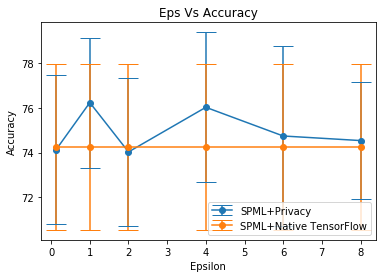
\includegraphics[width=\textwidth]{images/RR/nativeAccuracy.png}
         \caption{Accuracy}
         \label{fig:nativeRRAccuracyInference}
     \end{subfigure}
     \begin{subfigure}{0.5\textwidth}
         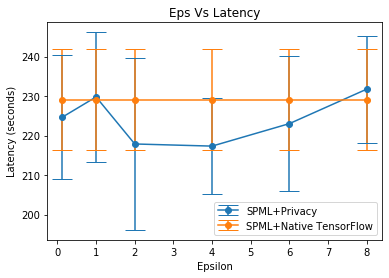
\includegraphics[width=\textwidth]{images/RR/nativeLatency.png}
         \caption{Latency}
         \label{fig:nativeRRLatencyInference}
     \end{subfigure}
        \caption{Randomized response - Training - Native mode without Intel SGX and SCONE}
     \begin{subfigure}{0.5\textwidth}
         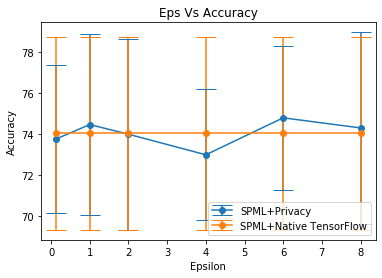
\includegraphics[width=\textwidth]{images/RR/simAccuracy.png}
         \caption{Accuracy}
         \label{fig:simRRAccuracyInference}
     \end{subfigure}
     \begin{subfigure}{0.5\textwidth}
         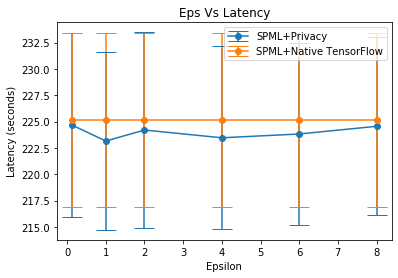
\includegraphics[width=\textwidth]{images/RR/simLatency.png}
         \caption{Latency}
         \label{fig:simRRLatencyInference}
     \end{subfigure}
        \caption{Randomized response - Training - Simulation mode without Intel SGX and with SCONE}
     \begin{subfigure}{0.5\textwidth}
         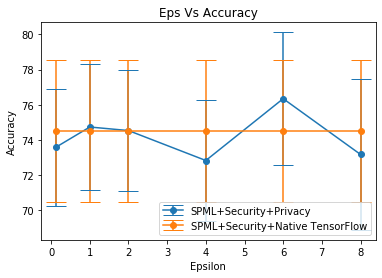
\includegraphics[width=\textwidth]{images/RR/hwAccuracy.png}
         \caption{Accuracy}
         \label{fig:hwRRAccuracyInference}
     \end{subfigure}
     \begin{subfigure}{0.5\textwidth}
         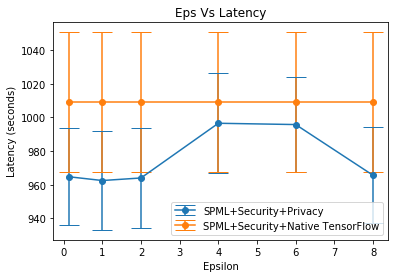
\includegraphics[width=\textwidth]{images/RR/hwLatency.png}
         \caption{Latency}
         \label{fig:hwRRLatencyInference}
     \end{subfigure}
        \caption{Randomized response - Training - Hardware mode with Intel SGX and SCONE}
\end{figure}




% -*- Mode: Latex -*-

\selectlanguage{american}
% \section*{\vfill{} \thispagestyle{empty} Declaration}
\section*{}\thispagestyle{empty}
\vspace{2.5cm}
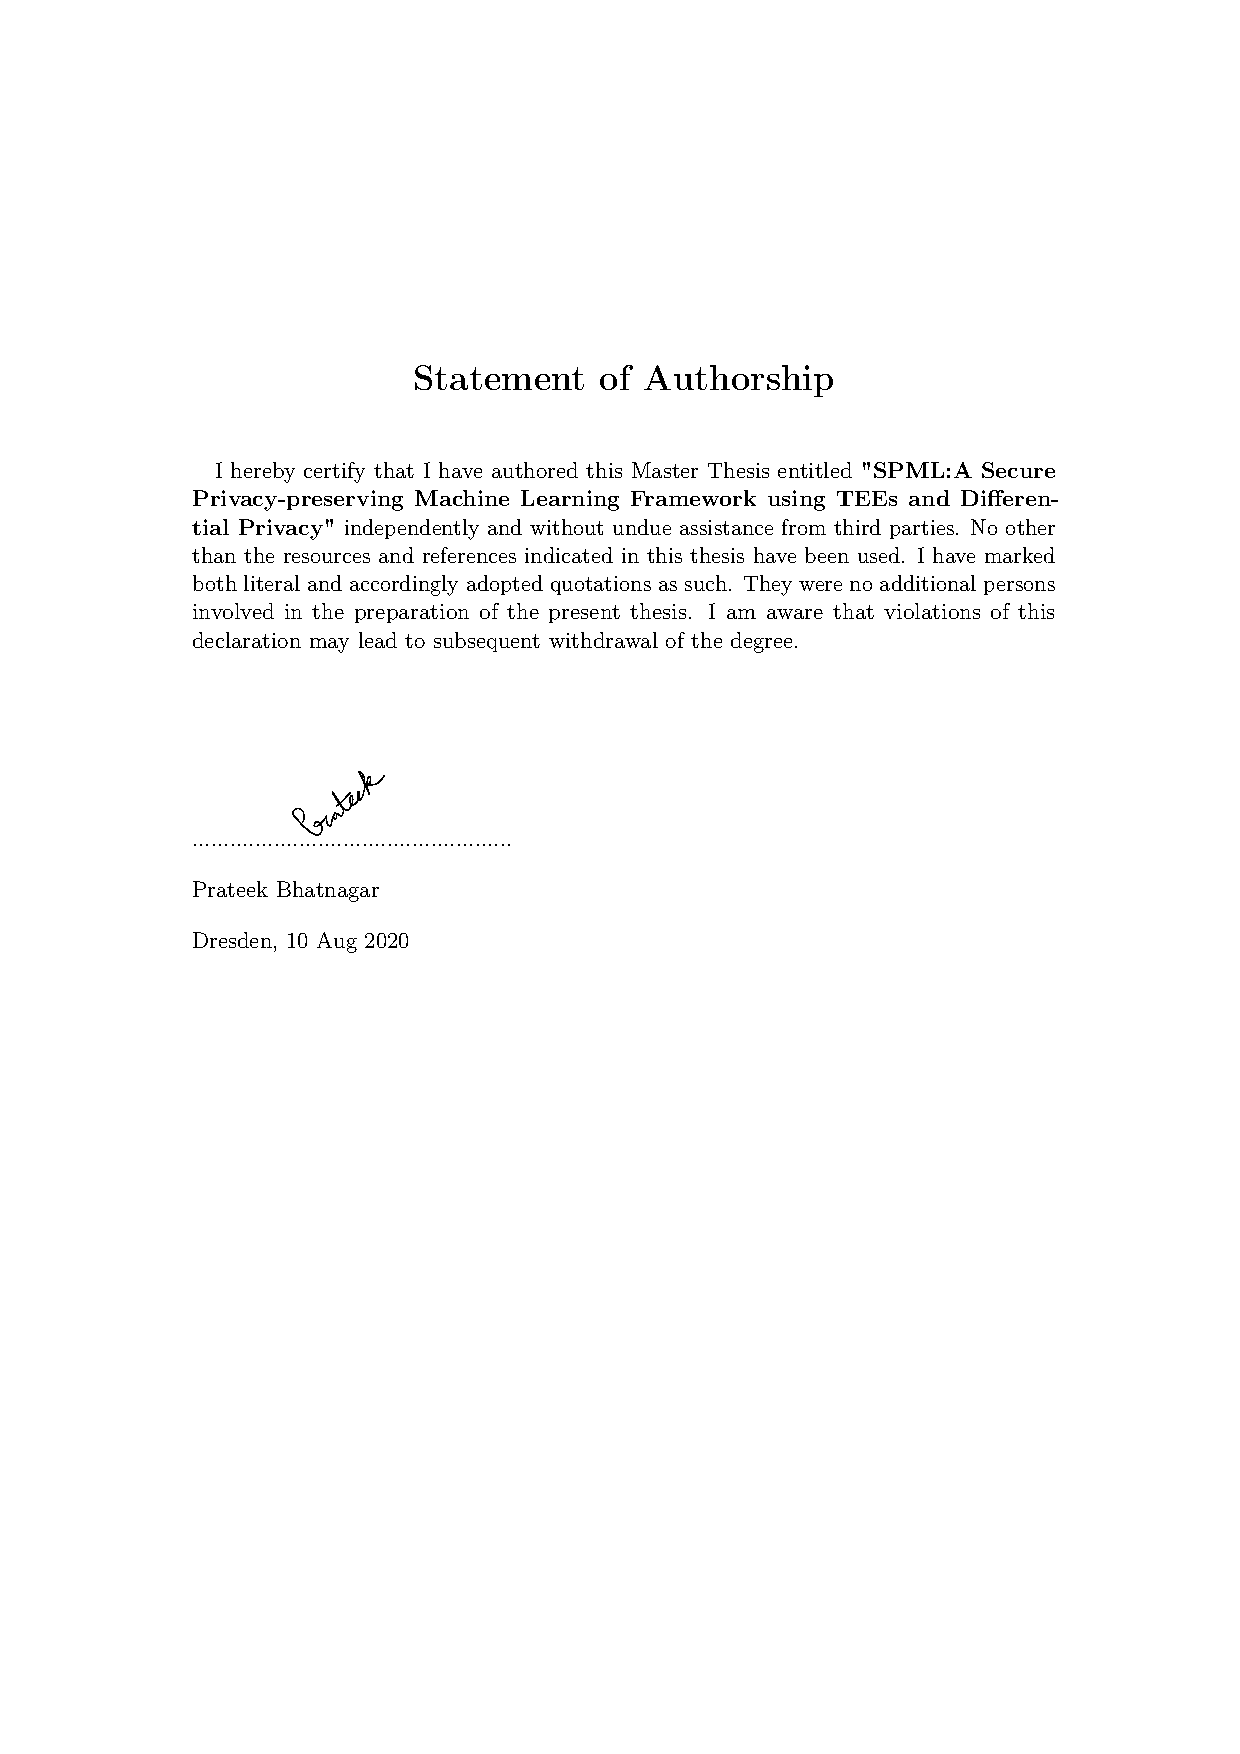
\includegraphics[width=\textwidth]{content/Disclaimer.pdf}
% \section*{Statement of Authorship}

\begin{center}
\textbf{\LARGE Statement of Authorship}
\end{center}
\medskip

I hereby certify that I have authored this Master Thesis
entitled \textbf{"SPML:A Secure Privacy-preserving Machine Learning Framework using TEEs and Differential Privacy"}
independently and without undue assistance from third parties.
No other than the resources and references indicated in this
thesis have been used. I have marked both literal and accordingly
adopted quotations as such. They were no additional persons involved
in the preparation of the present thesis. I am aware that
violations of this declaration may lead to subsequent withdrawal of
the degree.


\vspace{2.5cm}
\noindent ...................................................

\noindent Prateek Bhatnagar

\noindent Dresden, \printdate

\cleardoublepage
